\chapter{无延迟策略的模仿}
\label{chap:imitation_undelayed}

\section{引言}
本章首先考虑常值状态观测或动作执行延迟。
如\Cref{sec:related_works}所述，常值延迟相关文献主要集中于三个方向：增广方法、无记忆方法和基于模型的方法。
前一章探索了基于模型的方法。
本章探索一条新方向，源自一种简单而高效的方法（后文将展示其高效性）。
核心理念是通过模仿无延迟策略的行为学习延迟策略。
遵循模仿学习（imitation learning）文献的惯例，本章将执行模仿的策略称为学习器（learner），将被模仿的策略称为专家（expert）。
显然，延迟策略（学习器）可能无法精确模仿无延迟策略（专家），因为前者仅能访问增广状态，而无延迟策略可访问当前状态。
但期望在于，模仿所得策略与专家策略足够相似，从而其性能仍接近专家水平。

本文提出一种算法——基于数据集聚合的延迟模仿（Delayed Imitation with Dataset Aggregation, DIDA），该算法建立在模仿学习算法 \textsc{DAgger}~\cite{ross2011reduction} 基础之上（另见\Cref{subsec:dida_algo}）。
由于延迟加剧了学习器与专家之间状态分布的偏移，\textsc{DAgger} 尤为适用，因其在自身分布下表达模仿损失~\cite{osa2018algorithmic}。

在更详细地介绍该方法后，本文将证明 DIDA 在理论和实验上均取得优异结果。
在理论上，本文为 DIDA 所学策略相对于无延迟专家提供了紧致的性能保证（\Cref{sec:th_analysis_imitation}）。
在实验上，本文在广泛任务中测试 DIDA，与众多基线方法对比，并展示了其在最终性能和样本效率方面的优越性（\Cref{sec:exp_imitation}）。

最后，除常值整数延迟之外，本文提出 DIDA 的三种扩展。
通过对原始实现进行微小修改，将 DIDA 应用于非整数延迟并扩展了理论保证（\Cref{subsec:dida_non_int}）。
接着，为 DIDA 所学策略在随机延迟任务中测试的情形提供理论界，这是匿名状态观测或动作执行延迟的首个界（\Cref{subsec:stoch_delay_dida}）。
随后，详细阐述如何将 DIDA 针对给定延迟所学策略应用于更小延迟（\Cref{subsubsec:multi_delay_once_imitation}）。
所有扩展均经实验验证，结果令人满意。

\section{无延迟策略的模仿学习}

核心理念如\Cref{fig:imitation_delay_explanation}所示，即模仿无延迟专家在当前未观测状态上会执行的策略。
由于当前状态未知，只能根据增广状态计算其信念。
因此，延迟策略学习在信念分布下复制无延迟策略的动作。
使用 \textsc{DAgger}~\cite{ross2011reduction} 作为模仿学习算法，因其能够考虑专家与学习器策略之间的分布偏移，如\Cref{subsec:imitation_learning}所述。
这是一项重要性质，因为延迟加剧了状态分布的偏移。
该偏移将在\Cref{subsec:analysis_ismmdp}中详细讨论。

\begin{figure}[t]
    \centering
    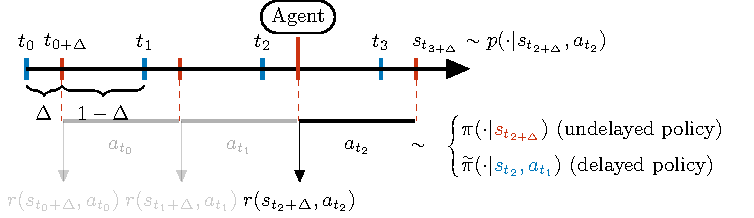
\includegraphics[labelimitation=dualitytrajectory]{img/thesis_plots_imitation.pdf}
    \caption{无延迟策略 $\pi$（专家）被延迟策略 $\delayedpolicy$（学习器）模仿的示意图。
    学习器仅能看到增广状态，对当前状态 $s_t$ 不可见。}
    \label{fig:imitation_delay_explanation}
\end{figure}


\subsection{轨迹的对偶性}
应用 \textsc{DAgger} 的重要前提是专家和学习器均能从环境中采样。
对于常值延迟 \gls{dmdp}，这得益于所谓轨迹的对偶性（duality of trajectories）。
一方面，在 \gls{mdp} 中，可通过忽略最新状态信息、向智能体提供过去状态及此后执行的动作序列来构造合成增广状态。
通过此方式，可在无延迟环境中从延迟策略采样。
另一方面，延迟环境中的智能体最终将观测到其当前状态\footnote{这在部分可观测马尔可夫决策过程（POMDP）中通常不成立。}。
得益于这一性质，延迟策略采样所得任意轨迹的概率均可按无延迟策略计算。
综上所述，一旦完成采样，轨迹既可自延迟策略视角分析，亦可自无延迟策略视角分析，无论该轨迹是如何采样的。
因此，常值延迟 \gls{dmdp} 满足将 \textsc{DAgger} 应用于模仿问题的前提。


\subsection{基于数据集聚合的延迟模仿（DIDA）}
\label{subsec:dida_algo}

\subsubsection{通用算法}
遵循 \textsc{DAgger} 框架（见\Cref{subsec:imitation_learning}），提出基于数据集聚合的延迟模仿（Delayed Imitation with Dataset Aggregation, DIDA）。
与 \textsc{DAgger} 类似，DIDA 通过跟随专家策略或学习器策略从环境中采样。
若选择专家，则在环境的当前状态上查询无延迟策略 $\pi$。若选择学习器策略，则从轨迹历史中合成构造增广状态，并将其输入延迟策略 $\delayedpolicy$。
实践中，这意味着需要维护一个近期历史缓冲区。
对于模仿步骤，DIDA 构建一个数据集 $\mathcal{D}=(x^{(i)},a_E^{(i)})_{0\le i\le N}$，其中包含增广状态 $x^{(i)}$ 与无延迟策略在当前未观测状态上所选动作 $a_E^{(i)}$ 的元组。
随后，延迟策略在 $\mathcal{D}$ 上训练，以在给定增广状态时复制专家的动作。
实际实现中，增广状态的存储可以高效完成。
事实上，两个连续增广状态中的大部分动作是相同的。
因此，只需存储状态-动作历史，并在训练时才构造增广状态即可。
DIDA 的算法如\Cref{algo:dida}所示。


\subsubsection{无无延迟环境时的 DIDA}
\label{subsubsec:dida_no_undelayed_env}
若无法访问可直接应用 DIDA 的无延迟环境，对该算法稍作修改即可使用。
当本应在未观测当前状态上查询无延迟策略时，可改为在最后观测到的状态上以无记忆方式查询无延迟策略（见\Cref{subsec:memoryless}）。
当 \textsc{DAgger} 的 $\beta$-routine 满足 $\beta_1=1, \beta_{i\ge 2}=0$（见\Cref{subsec:dida_algo}）时，这一点更为重要。
即仅第一次迭代使用无延迟策略（此时延迟策略尚未训练），后续迭代仅查询延迟策略。
需对\Cref{algo:dida}做两处修改。
首先，在第5行，将 $a_E\sim\pi(\cdot\vert s_{\delay+1})$ 替换为 $a_E\sim\pi(\cdot\vert s_{1})$。
其次，数据集 $\mathcal{D}$ 的填充方式应更改。
因为不需要专家以无记忆方式选择的动作。
相反，存储在 $\mathcal{D}$ 中的专家动作应对应于专家在未观测当前状态下选择的动作。
这意味着，在实践中，观察到增广状态 $x$ 后，智能体需等待 $\delay$ 步才能观察到当前未观测状态。
只有在那时，无记忆专家才能提供动作 $a_E$，与 $x$ 一同添加到数据集 $\mathcal{D}$ 中。
因此，\Cref{algo:dida} 的第10行必须相应延迟。
将 DIDA 的这一变体称为 memoryless-DIDA（M-DIDA）。


\subsubsection{DIDA 学习得到的策略}
\label{subsubsec:dida_policy_learnt}
在随机 \glspl{mdp} 中，未观测当前状态的信念支撑可能扩展到多个状态。DIDA 将学习在该分布下复制专家的动作。
形式上，完全模仿下 DIDA 的输出策略如下：
\begin{align}
    \delayedpolicy(a\vert x) = \int_{\statespace} \augmentedbelief(s\vert x) \pi(a\vert s)\de s.\label{eq:belief_pol}
\end{align}
值得注意的是，该策略可视为基于模型的策略，\Cref{pp:counter_example_belief_based} 适用于它。因此，存在某些 \glspl{mdp} 使得 DIDA 相比最优无延迟策略是次优的。后续\Cref{sec:th_analysis_imitation}的理论分析将表明，该策略在平滑 \glspl{mdp} 中仍然是高效的。

\Cref{eq:belief_pol} 中的策略是在完全模仿下获得的，然而实践中，取决于损失函数，该策略可能有所不同。下面给出两个例子。

\noindent\textbf{均方误差损失（Mean squared error loss）。}\indent 对于从 $\mathcal{D}$ 中采样的 $x$，若 DIDA 的模仿步骤满足，
\begin{align*}
    \argmin_{\vectorialform{\theta}\in\Theta} \int_{\statespace}\int_{\actionspace} (a-\delayedpolicy_{\vectorialform{\theta}}(x))^2 \pi(a\vert s) \augmentedbelief(s\vert x)\de a\de s,
\end{align*}
则输出策略为，
\begin{align*}
    \delayedpolicy_{\vectorialform{\theta}^\star}(x) = \expectedvalue_{s\sim \augmentedbelief(\cdot\vert x)}\left[ \expectedvalue_{a \sim\pi(\cdot \vert s)}[a]\right].
\end{align*}
即，该策略返回专家策略在信念上的均值。

\noindent\textbf{Kullback-Leibler 损失（Kullback-Leibler loss）。}\indent 对于从 $\mathcal{D}$ 中采样的 $x$，DIDA 学习到的策略满足：
\begin{align}
    &\argmin_{\vectorialform{\theta}\in\Theta} \int_{\statespace} \kullbackleiblerdivergence(\pi(\cdot \vert s) \Vert \delayedpolicy_{\vectorialform{\theta}}(\cdot \vert x)) \augmentedbelief(s\vert x)\de s\nonumber
    \\
    &= \argmin_{\vectorialform{\theta}\in\Theta} - \int_{\statespace} \int_{\actionspace} \pi(a \vert s) \log \delayedpolicy_{\vectorialform{\theta}}(a \vert x)) \augmentedbelief(s\vert x)\de a \de s\label{eq:indpt_theta}
    \\
    &= \argmin_{\vectorialform{\theta}\in\Theta}  - \int_{\actionspace}\int_{\statespace}  \pi(a \vert s) \log \delayedpolicy_{\vectorialform{\theta}}(a \vert x)) \augmentedbelief(s\vert x)\de s \de a\label{eq:fubini}
    \\
    &= \argmin_{\vectorialform{\theta}\in\Theta}  \int_{\actionspace} \int_{\statespace}  \pi(a \vert s) \augmentedbelief(s\vert x)\log\left(\augmentedbelief(s\vert x) \pi(a \vert x))\right)\de s\de a\nonumber
    \\
    &\qquad- \int_{\actionspace}\int_{\statespace}  \pi(a \vert s) \log \delayedpolicy_{\vectorialform{\theta}}(a \vert x)) \augmentedbelief(s\vert x)\de s\de a\label{eq:add_pas_depend_theta}
    \\
    &= \argmin_{\vectorialform{\theta}\in\Theta}  D_{KL}\left(\left.\int_{\statespace}\pi(\cdot \vert s)b(s\vert x)\de s \right\Vert \delayedpolicy_{\vectorialform{\theta}}(\cdot \vert x)\right) ,\nonumber
\end{align}
其中\Cref{eq:indpt_theta} 通过展开 KL 散度并注意到其中一项不依赖于 $\vectorialform{\theta}$ 得到；\Cref{eq:fubini} 由 Fubini 定理成立，因积分内的函数始终为负；\Cref{eq:add_pas_depend_theta} 通过添加一项不依赖于 $\vectorialform{\theta}$ 的项得到。



\begin{algorithm}[t]
\caption{基于 \textsc{DAgger} 的延迟模仿算法（DIDA）}\label{algo:dida}
\textbf{Inputs}
(un)delayed \gls{mdp} $\markovdecisionprocess$, undelayed expert $\pi$, $\beta$-routine, number of steps $N$, empty dataset $\mathcal{D}$.\\
\textbf{Outputs}: delayed policy $\delayedpolicy$
\begin{algorithmic}[1]
    \FOR{$\beta_i$ in $\beta$-routine}
        \FOR{$j$ in $\{1,\dots,N\}$}
            \IF{New episode}
                \STATE Initialize state buffer $( s_{1},s_{2}, \dots, s_{\delay+1})$ and action buffer $( a_{1},a_{2} \dots, a_{\delay})$
            \ENDIF
            \STATE Sample $a_E\sim\pi(\cdot\vert {{s}}_{\delay+1})$, set $a=a_E$ \label{ope:undelayed_sample}
            \IF{Random $u \sim U([0,1])\geq \beta_i$}
                \STATE Overwrite ${ a \sim\pi_I(\cdot\vert [{s}_{1},a_{1}, \dots, a_{\delay}])}$
            \ENDIF
            \STATE Aggregate dataset:
            $$\qquad \mathcal{D}\gets \mathcal{D} \cup ([{s}_{1}, a_{1}, \dots, a_{\delay}],a_E)$$
            \STATE Apply $a$ in $\markovdecisionprocess$ and get new state $s$
            \STATE Update buffers:
            $$\qquad ({s}_1,\dots,{s}_{\delay+1}) \gets ({s}_2,\dots,{s}_{\delay+1},s)$$
            $$\qquad  ({a}_1,\dots,{a}_{\delay}) \gets ({a}_2,\dots,{a}_{\delay},a)$$
            \ENDFOR
        \STATE Train $\delayedpolicy$ on $\mathcal{D}$
    \ENDFOR
\end{algorithmic}
\end{algorithm}



\subsection{非整数延迟}
\label{subsec:dida_non_int}
下面将前述算法扩展到非整数延迟情形。
然而，首先需要推导一些理论结果，以便扩展该框架。


\subsubsection{非整数延迟的理论}
注意到，即使延迟小于一个步长 $\delay\in (0,1)$，也需要增广状态 $x_t = (s_t,a_{t-1})\in \statespace \times \actionspace \eqqcolon \augmentedstatespace$。
这是因为在某个时刻 $t+\epsilon$（其中 $\epsilon\le\delay$）施加的动作仍然是上一时刻选择的动作 $a_{t-1}$。
在后续章节中，使用记号 "~$\integerpart{\ }$~" 表示实数的整数部分，"~$\fractionalpart{\ }$~" 表示其小数部分，"~$\lceil\ \rceil$~" 表示大于它的最小整数。
关于如何通过两个交错 \glspl{mdp} 构造非整数延迟环境，参见\Cref{subsec:non_int_delays}。
当 $\delay\in (0,1)$ 时，这些交错 \glspl{mdp} 为 $\markovdecisionprocess$ 和 $\markovdecisionprocess_\delay$。
当 $\delay>1$ 时，只需将第二个 \gls{mdp} 平移延迟的小数部分。因此，这两个 \glspl{mdp} 为 $\markovdecisionprocess$ 和 $\markovdecisionprocess_{\fractionalpart\delay}$。
第一个结果是，非整数延迟问题可以重新归结为 \gls{mdp}。

\begin{prop}
\label{pp:equivalent_mdp_non_int}
    设 $\delay\in\realnumbers[\ge0]$ 为一个（非）整数延迟，考虑一个在动作执行或状态观测上具有常值延迟 $\delay$ 的 \gls{dmdp} $\delayedmarkovdecisionprocess$。
    则可通过用最近的 $\lceil\delay\rceil$ 个动作增广状态，将该问题重新归结为 \gls{mdp}。
\end{prop}
\begin{proof}
    针对动作执行延迟证明此结果，状态观测延迟的证明可类似推导。
    构造一个 \gls{mdp} $\markovdecisionprocess$，使用增广状态空间 $\augmentedstatespace=\statespace\times\actionspace^{\lceil\delay\rceil}$ 作为其状态空间，使得对任意延迟策略，其在 $\markovdecisionprocess$ 中的回报等于在 $\delayedmarkovdecisionprocess$ 中的回报。
    对于增广状态 $x=(s,a_1,\dots,a_{\lceil\delay\rceil})$ 和 $x'=(s',a_1',\dots,a_{\lceil\delay\rceil}')$ in $\augmentedstatespace$，新的转移分布为：
    \begin{align*}
        \augmentedtransitionfunction(x'\vert x, a)\coloneqq
        p(s'\vert s,a_1)\delta_a(a_{\lceil\delay\rceil}')\prod_{i=1}^{\lceil\delay\rceil-1}\delta_{a_{i+1}}(a_{i}').
    \end{align*}
    注意，当 $\delay\notin \naturalnumbers$ 时，$p$ 的定义如\Cref{eq:def_p_non_int}所示：
    \begin{align}
        p(s'\vert s,a)=\int_{\statespace}   \augmentedbelief[1-\fractionalpart{\delay}](s'\vert z,a)\augmentedbelief[\fractionalpart{\delay}](z|s,a)\de z.
    \end{align}
    现在，对于 $x=(s,a_1,\dots,a_{\lceil\delay\rceil})$，期望奖励定义为，
    \begin{align*}
        \augmentedexpectedrewardfunction(x,a) = \expectedvalue_{z\sim \augmentedbelief(z\vert x)}[\expectedrewardfunction(z,a)].
    \end{align*}
    为完成证明，设 $\delayedpolicy$ 为 $\delayedmarkovdecisionprocess$ 的任意历史依赖策略。假设在时刻 $t$，$\delayedmarkovdecisionprocess$ 和 $\markovdecisionprocess$ 中观测到的状态与动作历史 $(s_0,a_0,\dots,s_{t},a_t,\dots,a_{t+\lceil\delay\rceil-1})\in\statespace^t\times\actionspace^{t+\lceil\delay\rceil}$\footnote{$\augmentedstatespace^t\times\actionspace^t$ 上的历史显然定义了 $\statespace^t\times\actionspace^{t+\lceil\delay\rceil}$ 上的一个历史。}相同。
    任何基于历史的策略智能体随后在 $\markovdecisionprocess$ 和 $\delayedmarkovdecisionprocess$ 中以相同概率选择下一个动作 $a_{t+\lceil\delay\rceil}$。
    在 $\delayedmarkovdecisionprocess$ 中，给定当前观测状态 $s_t$ 和其效果尚未显现的动作 $a_{t}$，智能体以概率 $p(s_{t+1}\vert s_t,a_{t})$ 观测到新状态 $s_{t+1}$。
    在 $\markovdecisionprocess$ 中，新增广状态中包含的状态 $s_{t+1}$ 同样根据设计从 $p(s_{t+1}\vert s_t,a_{t})$ 采样。
    因此，$t+1$ 时刻的历史也匹配。
    通过归纳，这对任意 $t'>t$ 均成立。
    只需以相同方式初始化这两个过程，即可使它们在 $\statespace$ 上具有相同的状态分布。
    由于历史相同，$\delayedmarkovdecisionprocess$ 和 $\markovdecisionprocess$ 中收集的奖励也由设计保证相等。
    这意味着任意延迟策略在两个过程中达到相同的回报。
\end{proof}

注意，为证明状态观测延迟的前述命题，需交换 $\markovdecisionprocess$ 和 $\markovdecisionprocess_{\fractionalpart\delay}$ 这两个 \glspl{mdp}。
事实上，考虑 $\delay\in(0,1)$；对于动作执行延迟，智能体看到当前状态 $s_t$，但其动作 $a_t$ 在 $t+\delay$ 时刻执行于状态 $s_{t+\delay}$。
对于状态观测延迟，若智能体的当前未观测状态也是 $s_t$，则最近观测到的状态将是 $s_{t-\delay}$，若 $\textstyle\delay\neq \frac{1}{2}$，该状态不属于 $\markovdecisionprocess_{\delay}$。
相反，如果将当前未观测状态置于 $s_{t+\delay}$，则延迟状态总是属于 $\markovdecisionprocess$。
总之，两个过程之间的区别在于智能体何时选择动作。
对于动作执行延迟，智能体在其当前状态属于 $\markovdecisionprocess$ 时选择动作；而对于状态观测延迟，智能体在其当前状态属于 $\markovdecisionprocess_{\delay}$ 时选择动作。
这种控制步长的偏移可通过\Cref{fig:non_int_delay_def}形象理解。

下面给出一个结果，表明与整数情形类似，动作执行延迟和状态观测延迟在非整数情形下也是等价的。
\begin{prop}
    设 $\delay\in\realnumbers[\ge0]$ 为一个（非）整数延迟。
    设 $\markovdecisionprocess$ 和 $\markovdecisionprocess_{\fractionalpart{\delay}}$ 是两个交错的 \glspl{mdp}，在此基础上定义两个常值延迟 \glspl{dmdp}：$\delayedmarkovdecisionprocess$ 在动作执行上延迟 $\delay$，$\delayedmarkovdecisionprocess'$ 在状态观测上延迟 $\delay$\footnote{首先固定 $\markovdecisionprocess$ 和 $\markovdecisionprocess_{\fractionalpart{\delay}}$ 确保两个 \glspl{dmdp} 中观测到的状态与执行动作时所处的状态相对应。否则，可以构造出动作延迟智能体观测 $s_t$ 并作用于 $s_{t+\delay}$，而状态延迟智能体观测 $s_{t-\delay}$ 并作用于 $s_t$ 的情形，此时会出现不匹配。}。
    则 $\delayedmarkovdecisionprocess$ 和 $\delayedmarkovdecisionprocess'$ 等价。
\end{prop}
\begin{proof}
    通过观察\Cref{pp:equivalent_mdp_non_int} 中构造的等价 \glspl{mdp} 相同，即可得证。
\end{proof}


\subsubsection{面向非整数延迟的 DIDA}
\label{subsubsec:dida_non_int}

现在将 DIDA 扩展到非整数情形。使用\Cref{subsec:non_int_delays} 中的记法，以两个交错 \glspl{mdp} $\markovdecisionprocess$ 和 $\markovdecisionprocess_\delay$ 定义非整数延迟。
与 DIDA 类似，第一步是学习一个无延迟策略。此处，无延迟策略在 $\markovdecisionprocess_\delay$ 中学习。
而延迟智能体观测到的状态将是 $\markovdecisionprocess$ 中的状态。
修改后的算法如\Cref{algo:dida_non_int} 所示。
与\Cref{algo:dida} 的主要区别在于，DIDA 必须记住最近的 $\lceil\delay\rceil$ 个动作。
此外，DIDA 还必须同时维护来自 $\markovdecisionprocess$ 和 $\markovdecisionprocess_\delay$ 的状态缓冲区，因为前者用于构造增广状态，后者用于计算无延迟专家的动作。
注意，DIDA 针对非整数延迟学习的策略仍然满足\Cref{eq:belief_pol}。

\begin{remark}
    类似思路也可用于上一节提出的算法。
    D-TRPO 可以调整，使其在观测 $\markovdecisionprocess$ 中状态的同时，学习 $\markovdecisionprocess_\delay$ 中的信念表示。
\end{remark}


\subsubsection{非整数延迟的时间 Lipschitz 性质}
为将下一节的理论扩展到非整数延迟，现将非整数延迟纳入 $L_T$-TLC 的定义中（见\Cref{def:time_lip}）。给定 $\delay\in(0,1)$，若 $\forall s,a\in \statespace\times\actionspace$，
\begin{align}
\label{eq:time_lip_non_int}
    \wassersteindistance(b_\delay(\cdot\vert s,a), \delta_s)\le \delay L_T.
\end{align}
则称 \gls{dmdp} 是 $L_T$-TLC 的。




\begin{algorithm}[t]
\caption{面向非整数延迟的 DIDA（$\delay\in\realnumbers[\ge0]$）}\label{algo:dida_non_int}
\textbf{Inputs}:
$\{\delay\}\coloneqq\delay-\lfloor\delay\rfloor$, \glspl{mdp} $\markovdecisionprocess$ and $\markovdecisionprocess_{\{\delay\}}$ obtained from continuous-time \gls{mdp}, undelayed expert $\pi$ trained on $\markovdecisionprocess_{\delay}$, $\beta$-routine, number of steps $N$, empty dataset $\mathcal{D}$.\\
\textbf{Outputs}: delayed policy $\pi_I$
\begin{algorithmic}[1]
    \FOR{$\beta_i$ in $\beta$-routine}
        \FOR{$j$ in $\{1,\dots,N\}$}
            \IF{New episode}
                \STATE Initialize state buffer $( s_{1},s_{1+\fractionalpart{\delay}}, \dots, s_{\lceil\delay\rceil},s_{\delay+1})$ and action buffer $( a_{0},a_{1} \dots, a_{\lfloor\delay\rfloor})$
            \ENDIF
            \STATE Sample $a_E\sim\pi(\cdot\vert {{s}}_{\delay+1})$, set $a=a_E$
            \IF{Random $u \sim U([0,1])\geq \beta_i$}
                \STATE Overwrite ${ a \sim\delayedpolicy(\cdot\vert [{s}_{1},a_{0}, \dots, a_{\lfloor\delay\rfloor}])}$
            \ENDIF
            \STATE Aggregate dataset:
            $$\mathcal{D}\leftarrow \mathcal{D} \cup ([{s}_{1}, a_{0},a_2, \dots, a_{\lfloor\delay\rfloor}],a_E)$$
            \STATE Apply $a$ at $s_{\delay+1}$ and get new states $(s_{\lceil\delay\rceil+1},s_{\delay+2})$
            \STATE Update buffers:
            $$(s_{1}, s_{1+\fractionalpart{\delay}}, \dots, s_{\lceil\delay\rceil},s_{\delay+1}) \leftarrow ( s_{2},s_{2+\fractionalpart{\delay}}, \dots, s_{\lceil\delay\rceil+1},s_{\delay+2})$$
            $$({a}_0,\dots, a_{\lfloor\delay\rfloor}) \leftarrow ({a}_1,\dots,a_{\lfloor\delay\rfloor},a)$$
            \ENDFOR
        \STATE Train $\delayedpolicy$ on $\mathcal{D}$
    \ENDFOR
\end{algorithmic}
\end{algorithm}



\subsection{同时学习多重延迟的 DIDA}
\label{subsubsec:multi_delay_once_imitation}

与\Cref{subsec:multi_delay_once_belief} 中相同的思想可应用于 DIDA。
针对延迟 $\delay>0$ 学习的策略，可通过模拟 $\delay$ 的延迟，在具有较小延迟 $0<\delay'<\delay$ 的环境中执行。
\Cref{sec:exp_imitation} 中的实验将展示该思路的有效性。

\section{DIDA 理论分析}
\label{sec:th_analysis_imitation}

本节理论分析旨在实现两个目标。
首先，为延迟策略与无延迟策略之间的性能差异提供界。
这些界将依赖于环境平滑性假设（见\cref{{subsec:smooth_mdp}}）。
其次，研究这些界有助于理解哪些无延迟专家更适于在延迟环境中被模仿。


\subsection{延迟与无延迟性能的比较}
\label{subsec:compare_delayed_undelayed}

在直接给出理论结果之前，有必要澄清一点。
需要比较延迟策略和无延迟策略的价值函数，然而它们的输入空间不同。
具体而言，延迟策略 $\delayedpolicy$ 的输入空间为 $\augmentedstatespace=\statespace\times\actionspace^\delay$，而无延迟策略的输入空间为 $\statespace$。
下文详述文献中提出的两种比较方式。

\subsubsection{弱随机马尔可夫决策过程中的比较}
比较延迟策略与无延迟策略的一种可能方式由 \cite{walsh2009learning} 提出。
其思想源于以下观察：若 \gls{dmdp} 源自确定性 \gls{mdp}，则它们有相同的最优性能（直到\Cref{subsec:delay_init} 中提到的延迟初始化偏移）。
这易于理解：利用环境的确定性模型计算当前状态后，智能体可选择无延迟策略在该状态下推荐的动作。显然，困难在于学习 \gls{mdp} 的模型。
为扩展这一比较，\cite{walsh2009learning} 考虑了所谓的弱随机（mildly stochastic）\gls{mdp}，即满足如下条件的 \gls{mdp}：
\begin{align*}
    \exists \epsilon \text{ s.t. } \forall (s,a)\in\statespace\times\actionspace, \exists s', p(s'\vert s,a)\geq 1-\epsilon.
\end{align*}
由于这些 \glspl{mdp} 仅是弱随机的，可按上述方式针对 \gls{mdp} 的确定性近似学习最优延迟策略。
记 $\widehat{V}^{\pi}$ 为无延迟策略在 \gls{mdp} 确定性近似中的价值函数，则有 \cite[Theorem~3]{walsh2009learning}：
\begin{align*}
    \lVert \widehat{V}^{\pi}-{V}^{\pi}\rVert_{\infty}\leq \frac{\gamma\epsilon \maximumreward}{(1-\gamma)^2},
\end{align*}
其中 ${V}^{\pi}$ 是同一策略 $\pi$ 在无延迟 \gls{mdp} 中的价值函数。
注意这两个价值函数的输入空间均为 $\statespace$。
另一个值得注意的观察是，结果对有效时域 $\textstyle\frac{1}{1-\gamma}$ 呈二次依赖关系。
弱随机性假设相当强，本文将为更弱的假设提供结果。

\subsubsection{基于信念分布的比较}
另一种方法的优势在于可适用于任意 \gls{mdp}，由 \cite{agarwal2021blind} 提出。
对于给定增广状态 $x\in\augmentedstatespace$，作者比较了延迟策略的价值函数 $V^{\delayedpolicy}(x)$ 与无延迟策略在给定 $x$ 下信念的期望价值函数 $\textstyle\expectedvalue_{s\sim \augmentedbelief(\cdot\vert x)}[V^{\pi}(s)]$。
作者提出学习一种延迟策略，该策略选择的动作最大化无延迟策略 Q 函数在信念分布下的期望。
假设动作空间基数有限 $\cardinal{\actionspace}$，延迟策略 $\delayedpolicy$ 相对于最优策略 $\optimalpolicy$ 具有如下保证 \cite[Theorem~1]{agarwal2021blind}：
\begin{align*}
    V^\delayedpolicy(x) \ge \expectedvalue_{s\sim \augmentedbelief(\cdot\vert x)}[V^{\optimalpolicy}(s)] - \frac{\maximumreward}{(1-\gamma)^2}\left(1-\frac{1}{\cardinal{\actionspace}}\right)
\end{align*}
再次注意对有效时域的二次依赖关系。
在本文的分析中，将比较相同量，同时增加对底层 \gls{mdp} 平滑性的假设。




\subsection{常值延迟性能损失的上界}
\label{subsec:imitation_upper_bound}
在理论部分的余下内容中，假设底层 \gls{mdp} 是平滑的。具体而言，需要 \gls{mdp} 是 $(L_P,L_r)$-LC 的（见\Cref{def:lip_mdp}），且专家的无延迟策略是 $L_\pi$-LC 的（见\Cref{def:lip_policy}）。
此外，还需要其 Q 函数是 $L_Q$-LC 的\footnote{在某些情形下，这可由前两个假设推出，见\Cref{th:lip_Q_function}。}。
这些平滑性保证的优点在于排除了诸如\Cref{pp:counter_example_belief_based} 中的病态例子。
然而，该设定仍然是现实的，因为许多物理系统是 Lipschitz 的。

为给出上界的主要结果，首先推导延迟情形下性能差异引理~\cite[Lemma~6.1]{kakade2002approximately} 的改编版本。
该结果本身可能对延迟文献有用。
该结果曾在 \cite[Equation~32]{agarwal2021blind} 中针对整数延迟独立推导，但本文给出一个更通用的版本，适用于延迟 $\delay\in\realnumbers[\ge0]$。
下文中，记 $\discountedstateoccupancydistribution[x][\delayedpolicy]$ 为延迟策略 $\delayedpolicy$ 从增广状态 $x$ 出发在增广状态空间 $\augmentedstatespace$ 上的折扣状态占据分布。


\begin{lemma}
[延迟性能差异引理（Delayed Performance Difference Lemma）]
\label{lem:perf_diff_lem}
    对于某些 $\delay\in\realnumbers[\ge0]$，设 $\pi$ 为无延迟策略，$\delayedpolicy$ 为同一底层 \gls{mdp} $\markovdecisionprocess$ 上的 $\delay$-延迟策略。
    则 $\forall x\in\mathcal{X}$，
    \begin{align*}
        \expectedvalue_{s\sim \augmentedbelief(\cdot\vert x)}[V^{\pi}(s)] - V^{\delayedpolicy}(x)
        = \frac{1}{1-\gamma}
        \quad\expectedvalue_{x'\sim \delayeddiscountedstateoccupancydistribution[x][\delayedpolicy]} \left[ \expectedvalue_{s\sim \augmentedbelief(\cdot\vert x')}[V^{\pi}(s)] -  \expectedvalue_{\substack{s\sim \augmentedbelief(\cdot\vert x')\\a\sim \delayedpolicy(\cdot\vert x')}}[Q^{\pi}(s,a)] \right].
    \end{align*}
\end{lemma}
\begin{proof}
    首先证明整数延迟下的结果。

    \noindent\textbf{整数延迟。}\indent 考虑 $\delay\in\naturalnumbers$，$x\in\augmentedstatespace$，设
    \begin{align*}
        I(x)=\expectedvalue_{s\sim \augmentedbelief(\cdot\vert x)}[V^{\pi}(s)] - V^{\delayedpolicy}(x).
    \end{align*}
    通过对 $I$ 加上并减去同一量，得到：
    \begin{align*}
        I(x)
        &= \underbrace{\expectedvalue_{s\sim \augmentedbelief(\cdot\vert x)}[V^{\pi}(s)] - \expectedvalue_{\substack{s\sim \augmentedbelief(\cdot\vert x)\\a\sim \delayedpolicy(\cdot\vert x)}}\left[r(s,a) + \gamma \expectedvalue_{s'\sim p(\cdot\vert s,a)}[V^{\pi}(s')]\right]}_{\eqcolon A}
        \\
        &\quad + \underbrace{\expectedvalue_{\substack{s\sim \augmentedbelief(\cdot\vert x)\\a\sim \delayedpolicy(\cdot\vert x)}}\left[r(s,a) + \gamma \expectedvalue_{s'\sim p(\cdot\vert s,a)}[V^{\pi}(s')]\right] - V^{\delayedpolicy}(x)}_{\eqcolon B}.
    \end{align*}
    然后分析上式中的每一项。首先，
    \begin{align*}
        A = \expectedvalue_{s\sim \augmentedbelief(\cdot\vert x)}[V^{\pi}(s)] - \expectedvalue_{\substack{s\sim \augmentedbelief(\cdot\vert x)\\a\sim \delayedpolicy(\cdot\vert x)}}\left[Q^{\pi}(s,a)\right].
    \end{align*}
    其次，由于 $V^{\delayedpolicy}(x) = \expectedvalue_{\substack{s\sim \augmentedbelief(\cdot\vert x)\\a\sim \delayedpolicy(\cdot\vert x)}}\left[r(s,a)\right]+ \gamma \expectedvalue_{\substack{x'\sim \augmentedtransitionfunction(\cdot\vert x,a)\\a\sim \delayedpolicy(\cdot\vert x)}}[V^{\delayedpolicy}(x')]$，则，
    \begin{align*}
        B &= \gamma\expectedvalue_{\substack{s\sim \augmentedbelief(\cdot\vert x)\\a\sim \delayedpolicy(\cdot\vert x)}}\left[ \expectedvalue_{s'\sim p(\cdot\vert s,a)}[V^{\pi}(s')]\right] - \gamma \expectedvalue_{\substack{x'\sim \augmentedtransitionfunction(\cdot\vert x,a)\\a\sim \delayedpolicy(\cdot\vert x)}}[V^{\delayedpolicy}(x')].
    \end{align*}
    注意，
    \begin{align}
    \label{eq:perf_diff_lem_equiv_belief}
        \int_{\statespace} \augmentedbelief(s\vert x)p(s'\vert s,a)\de s = \int_{\augmentedstatespace}\augmentedtransitionfunction(x'\vert x,a)\augmentedbelief(s'\vert x')\de x'.
    \end{align}
    这意味着，给定当前增广状态 $x$ 和某动作 $a$，下一个未观测当前状态为 $s'$ 的概率可通过两种方式获得：要么先以当前未观测状态 $s$ 为条件，要么以下一个增广状态 $x'$ 为条件。
    由此得到，
    \begin{align*}
        B &= \gamma \expectedvalue_{\substack{x'\sim \augmentedtransitionfunction(\cdot\vert x,a)\\a\sim \delayedpolicy(\cdot\vert x)}}\left[\expectedvalue_{s\sim \augmentedbelief(\cdot\vert x')}[V^{\pi}(s')] - V^{\delayedpolicy}(x') \right]
        \\
        &= \gamma \expectedvalue_{\substack{x'\sim \augmentedtransitionfunction(\cdot\vert x,a)\\a\sim \delayedpolicy(\cdot\vert x)}}\left[I(x')\right],
    \end{align*}
    通过识别量 $I$。现在，如同原始引理，迭代此结果：
    \begin{align}
        I(x) &= \sum_{t=0}^\infty \gamma^t \expectedvalue_{\substack{x_{t+1}\sim \augmentedtransitionfunction(\cdot\vert x_t,a_t)\\a_t\sim \delayedpolicy(\cdot\vert x_t)}}\left[\left. \expectedvalue_{s\sim \augmentedbelief(\cdot\vert x_t)}[V^{\pi}(s)] - \expectedvalue_{\substack{s\sim \augmentedbelief(\cdot\vert x_t)\\a\sim \delayedpolicy(\cdot\vert x_t)}}[Q^{\pi}(s,a)] \right\vert x_0=x \right]\nonumber
        \\
        &= \frac{1}{1-\gamma}\expectedvalue_{x'\sim \delayeddiscountedstateoccupancydistribution[x][\delayedpolicy]}\left[ \expectedvalue_{s\sim \augmentedbelief(\cdot\vert x')}[V^{\pi}(s)] - \expectedvalue_{\substack{s\sim \augmentedbelief(\cdot\vert x')\\a\sim \delayedpolicy(\cdot\vert x')}}[Q^{\pi}(s,a)] \right],\label{eq:state_distrib_reco}
    \end{align}
    其中\Cref{eq:state_distrib_reco} 由策略 $\delayedpolicy$ 的折扣增广状态占据分布定义得到（见\Cref{def:discounted_state_distrib}）。
    因此，证明了 $\delay\in\naturalnumbers$ 下的结果。

    \noindent\textbf{非整数延迟。}\indent 为证明清晰起见，假设 $\delay\in(0,1)$，但 $\delay\in\realnumbers[\ge0]$ 的一般结果可由此轻松导出。
    注意此时信念的定义如\Cref{subsec:non_int_delays} 所示。
    前述整数延迟的证明可顺利应用于非整数延迟。
    唯一可能不易直接推导的步骤是\Cref{eq:perf_diff_lem_equiv_belief}。
    因此，下面详述该步骤。
    对于 $x_t=(s_t,a_{t-1}), x_{t+1}=(s_{t+1},a_t)\in\augmentedstatespace$，
    \begin{align}
        &\int_{\statespace} \augmentedbelief(s_{t+\delay}\vert x_t)p(s_{t+1+\delay}\vert s_{t+\delay},a)\de s_{t+\delay}\nonumber
        \\
        &\qquad=\int_{\statespace} \augmentedbelief(s_{t+\delay}\vert x_t) \int_{\statespace}  \augmentedbelief(s_{t+1+\delay}\vert s_{t+1},a) b_{1-\delay}(s_{t+1}\vert s_{t+\delay},a)\de s_{t+1}\de s_{t+\delay} \label{eq:use_def_p_non_int}
        \\
        &\qquad= \int_{\statespace} \augmentedbelief(s_{t+1+\delay}\vert s_{t+1},a)\int_{\statespace} \augmentedbelief(s_{t+\delay}\vert x_t)b_{1-\delay}(s_{t+1}\vert s_{t+\delay},a)\de s_{t+\delay}\de s_{t+1} \nonumber
        \\
        &\qquad= \int_{\statespace} \augmentedbelief(s_{t+1+\delay}\vert s_{t+1},a)\int_{\statespace} \augmentedbelief(s_{t+\delay}\vert s_t,a_{t-1})b_{1-\delay}(s_{t+1}\vert s_{t+\delay},a)\de s_{t+\delay}\de s_{t+1} \nonumber
        \\
        &\qquad= \int_{\actionspace} \int_{\statespace} \augmentedbelief(s_{t+1+\delay}\vert s_{t+1},a_{t}) \delta_{a}(a_{t})\nonumber
        \\
        &\qquad\quad\int_{\statespace} \augmentedbelief(s_{t+\delay}\vert s_t,a_{t-1}) b_{1-\delay}(s_{t+1}\vert s_{t+\delay},a)\de s_{t+\delay}\de s_{t+1}\de a_{t}\nonumber
        \\
        &\qquad= \int_\augmentedstatespace \augmentedbelief(s_{t+1+\delay}\vert x_{t+1})\tilde p(x_{t+1}\vert x_t, a)\de x_{t+1}\label{eq:def_aug_mdp_p_non_int}.
    \end{align}
    \Cref{eq:use_def_p_non_int} 由\Cref{eq:def_p_non_int} 中 $p$ 的定义得到，\Cref{eq:def_aug_mdp_p_non_int} 通过识别增广 \gls{mdp} 中的转移得到。
\end{proof}


下面陈述本章的主要结果。
该结果不仅对 DIDA 有价值，对任何满足\Cref{eq:belief_pol} 的策略均有价值。
\glspl{dmdp} 的平滑性是证明的关键要素。

\begin{thm}
\label{th:perf_diff_bound}
    设 $\markovdecisionprocess$ 是 $(L_P,L_r)$-LC 的 \gls{mdp}，$\pi$ 是 $L_\pi$-LC 的无延迟策略。进一步假设 $Q^{\pi}$ 是 $L_Q$-LC 的\footnote{证明仅需 $Q^{\pi}$ 在第二个参数上的 Lipschitz 性质。}。
    设 $\delay\in\realnumbers[\ge0]$，并考虑满足\Cref{eq:belief_pol} 的 $\delay$-延迟策略 $\delayedpolicy$。
    则 $\forall x\in\mathcal{X}$，
    \begin{align*}
        \expectedvalue_{s\sim \augmentedbelief(\cdot\vert x)}&[V^{\pi}(s)] - V^{\delayedpolicy}(x) \leq \frac{L_Q L_\pi}{1-\gamma} \sigma_b^x,
    \end{align*}
    其中
    \begin{align*}
        \sigma_b^x = \expectedvalue_{\substack{x'\sim \delayeddiscountedstateoccupancydistribution[x][\delayedpolicy]\\ s,s'\sim \augmentedbelief(\cdot\vert x')}}\left[ \distance_{\statespace}(s,s') \right].
    \end{align*}
\end{thm}
\begin{proof}
    本证明无需区分整数和非整数延迟。
    设 $\delay\in\realnumbers[\ge0]$。由\Cref{lem:perf_diff_lem}，对于某些 $x \in \augmentedstatespace$，
    \begin{align*}
        \expectedvalue_{s\sim \augmentedbelief(\cdot\vert x)}&[V^{\pi}(s)] - V^{\delayedpolicy}(x)
        = \frac{1}{1-\gamma} \expectedvalue_{x'\sim \delayeddiscountedstateoccupancydistribution[x][\delayedpolicy]} \bigg[\underbrace{ \expectedvalue_{s\sim \augmentedbelief(\cdot\vert x')}[V^{\pi}(s)] -  \expectedvalue_{\substack{s\sim \augmentedbelief(\cdot\vert x')\\a\sim \delayedpolicy(\cdot\vert x')}}[Q^{\pi}(s,a)]}_{A(x')} \bigg].
    \end{align*}
    关注项 $A(x')$。有，
    \begin{align}
        A(x')
        &= \expectedvalue_{s\sim \augmentedbelief(\cdot\vert x')}\left[\expectedvalue_{\substack{a_1\sim\pi(\cdot\vert s) \\a_2\sim \delayedpolicy(\cdot\vert x')}}\left[ Q^{\pi}(s,a_1) -  Q^{\pi}(s,a_2) \right]\right]\nonumber
        \\
        &\leq L_Q \expectedvalue_{s\sim \augmentedbelief(\cdot\vert x')} \left[ \wassersteindistance(\pi(\cdot\vert s)
        \Vert \delayedpolicy(\cdot\vert x') ) \right],\label{eq:partial_res_v}
    \end{align}
    其中结果由应用\Cref{pp:expected_q_bound} 得到。
    最后一步是使用 $\sigma_b^x$ 对
    $\expectedvalue_{s\sim \augmentedbelief(\cdot\vert x')} \left[ \wassersteindistance(\pi(\cdot\vert s) \Vert \delayedpolicy(\cdot\vert x') ) \right]$ 进行上界估计。因此，
    \begin{align}
         \wassersteindistance(\pi(\cdot\vert s) \Vert \delayedpolicy(\cdot\vert x') )
        &= \sup_{\left\Vert f\right\Vert_L\leq 1}\left\vert\int_{\actionspace} f(a)(\pi(a\vert s)-\delayedpolicy(a\vert x')) \de a\right\vert \nonumber
        \\
        &= \sup_{\left\Vert f\right\Vert_L\leq 1}\left\vert\int_{\actionspace} f(a)(\pi(a\vert s)-\int_{\statespace}\pi(a\vert s')\augmentedbelief(s'\vert x')\de s') \de a\right\vert \label{eq:def_pidel}
        \\
        &\leq  \int_{\statespace} \augmentedbelief(s'\vert x') \sup_{\left\Vert f\right\Vert_L\leq 1}\left\vert\int_{\actionspace} f(a)(\pi(a\vert s)-\pi(a\vert s')) \de a \right\vert \de s' \label{eq:fub_ton_sigma}
        \\
        &\leq \int_{\statespace} \augmentedbelief(s'\vert x') \wassersteindistance(\pi(\cdot\vert s) \Vert \pi(\cdot\vert s') ) \de s'\nonumber
        \\
        &\leq L_\pi \int_{\statespace} \augmentedbelief(s'\vert x')  \distance_{\statespace}(s,s') \de s'
        \label{eq:lip_expert_pol}
        ,
    \end{align}
    其中\Cref{eq:def_pidel} 由\Cref{eq:belief_pol} 得到，\Cref{eq:fub_ton_sigma} 由 Fubini-Tonelli 定理得到，\Cref{eq:lip_expert_pol} 由 $\pi$ 的 Lipschitz 性质得到。
    将此结果代入\Cref{eq:partial_res_v} 即得结论。
\end{proof}

为使该结果更具实际解释性，提供两种方式进一步约束非常见项 $\sigma_b^x$，每种方式引入一个新的假设。
第一个结果假设 \gls{mdp} 具有时间 Lipschitz 性质（见\Cref{def:time_lip}）。

\begin{coroll}
\label{cor:perf_diff_bound_tlc}
    若\Cref{th:perf_diff_bound} 的假设成立，且此外 \gls{mdp} 是 $L_T$-TLC 的，则 $\forall x\in\mathcal{X}$，
    \begin{align*}
        \expectedvalue_{s\sim \augmentedbelief(\cdot\vert x)}&[V^{\pi}(s)] - V^{\delayedpolicy}(x) \leq \frac{2 \delay L_T L_Q L_\pi}{1-\gamma}.
    \end{align*}
\end{coroll}
\begin{proof}
    将\Cref{lem:bound_sigma_tlc} 应用于\Cref{th:perf_diff_bound} 即得结果。
\end{proof}

该结果清晰表明，性能差异的界与延迟呈线性关系。
该界的一个关键局限性在于，当 \gls{mdp} 变为确定性时，它不会趋于 0。事实上，如\Cref{subsec:compare_delayed_undelayed} 所述，在这种情况下，最优延迟回报应与无延迟回报匹配。
下面给出的 \Cref{th:perf_diff_bound} 的第二个推论则没有这一局限性。

\begin{coroll}
\label{cor:perf_diff_bound_eucl}
    若\Cref{th:perf_diff_bound} 的假设成立，且此外 $\statespace\subseteq\realnumbers^n$ 配备欧几里得范数，则 $\forall x\in\mathcal{X}$，
    \begin{align*}
        \expectedvalue_{s\sim \augmentedbelief(\cdot\vert x)}[V^{\pi}(s)] - V^{\delayedpolicy}(x) \leq
        \frac{\sqrt{2} L_Q L_\pi}{1-\gamma}
        \expectedvalue_{x'\sim \delayeddiscountedstateoccupancydistribution[x][\delayedpolicy]}\left[\sqrt{ \variance_{s\sim \augmentedbelief(\cdot\vert x')}(s\vert x')}\right].
    \end{align*}
\end{coroll}
\begin{proof}
    将\Cref{lem:bound_sigma_eucl} 应用于\Cref{th:perf_diff_bound} 即得结果。
\end{proof}

为评估这些界的质量，下面给出性能差异的下界结果。


\subsection{常值延迟性能损失的下界}
本小节通过展示在相同平滑性假设下，当专家的无延迟策略为最优时，\Cref{cor:perf_diff_bound_eucl} 与一个下界在常数项内匹配，从而增加其意义。

\begin{thm}
\label{th:lb_tight}
设 $L_\pi>0$，$L_{Q}>0$，$\delay\in\realnumbers[\ge0]$。
则存在一个 \gls{mdp}，其最优 $L_\pi$-LC 策略 $\optimalpolicy$ 的价值函数在第二个参数上是 $L_{Q}$-LC 的，但对任意 $\delay$-延迟策略 $\delayedpolicy$ 和 $x\in\augmentedstatespace$，
    \begin{align*}
        \expectedvalue_{s\sim \augmentedbelief(\cdot\vert x)}[\optimalstatevaluefunction(s)] - V^{\delayedpolicy}(x) &\geq
        \frac{\sqrt 2}{\sqrt \pi}\frac{ L_{Q}L_\pi}{1-\gamma}
        \expectedvalue_{x'\sim \delayeddiscountedstateoccupancydistribution[x][\delayedpolicy]}\left[\sqrt{ \variance_{s\sim \augmentedbelief(\cdot|x')}(s|x')}\right],
    \end{align*}
    其中 $\optimalstatevaluefunction$ 为最优无延迟策略的价值函数。
\end{thm}
\begin{proof}
    对于给定的 $L_\pi>0$，$L_{Q}>0$ 和 $\delay\in\realnumbers[\ge0]$，设计一个 \gls{mdp} $\markovdecisionprocess=(\statespace,\actionspace, \transitionfunction, \rewardfunction, \initialstatedistribution)$ 使得：$\statespace=\realnumbers$；$\actionspace=\realnumbers$；其转移函数为
    \begin{align*}
        \transitionfunction(s'\vert s,a)=\mathcal N\left(s';\; s+\frac{a}{L_\pi},\sigma^2\right),
    \end{align*}
    即 $s'=s+\frac{a}{L_\pi}+\varepsilon$，其中 $\varepsilon \sim \mathcal N (0,\sigma^2)$；
    其奖励函数为
    \begin{align*}
        \expectedrewardfunction(s,a)=\expectedvalue[\rewardfunction(s,a)] = -L_r\left\vert s+\frac{a}{L_\pi}\right\vert,
    \end{align*}
    其中 $L_r:=L_Q L_\pi$。
    在 $\expectedrewardfunction$ 的定义中使用 $L_Q$，因为后文将证明这正是 $\optimalstateactionvaluefunction$ 的 Lipschitz 常数。
    注意 $\forall (s,a)\in\statespace\times\actionspace,\;r(s,a)\le0$，但策略 $\optimalpolicy(a\vert s)=\delta_{-L_\pi s}(a)$ 对任意状态-动作对 $(s,a)$ 获得奖励 $0$。
    这意味着 $\optimalstatevaluefunction=0$ 处处成立。

    现在证明 Q 函数是 Lipschitz 的，
    \begin{align*}
        \optimalstateactionvaluefunction(s,a)&=-L_r\left\vert s+\frac{a}{L_\pi}\right\vert + \gamma \int_{\realnumbers} \optimalstatevaluefunction(s')\ p(s'\vert s,a)\de s'
        \\
        &= -L_r\left\vert s+\frac{a}{L_\pi}\right\vert
        \\
        &=-L_{Q}\left\vert L_\pi s+a\right\vert.
    \end{align*}
    因此，$\optimalstateactionvaluefunction$ 在第二个参数上是 $L_Q$-LC 的。

    现在研究 $\delay$-延迟策略 $\delayedpolicy$ 的情形。
    对于给定时间步 $t$，未观测当前状态为
    \begin{align*}
        s_t=\underbrace{s_{t-\delay}+\sum_{\tau=t-\delay}^{t-1} \frac{a_\tau}{L_\pi}}_{\eqqcolon \phi(x_t)}+\underbrace{\sum_{\tau=t-\delay}^{t-1} \varepsilon_\tau}_{\eqqcolon\epsilon}.
    \end{align*}
    上面定义了两个量。第一个 $\phi(x_t)$ 是增广状态 $x_t\in\augmentedstatespace$ 的确定性函数。
    第二个 $\epsilon$ 是服从分布 $\mathcal N(0,\delay\sigma^2)$ 的随机变量。
    利用这些量，可以定义增广奖励为，
    \begin{align*}
        \augmentedexpectedrewardfunction (x_t,a)
        &= -L_r\expectedvalue\left[\Big\vert s_t+\frac{a}{L_\pi}\Big\vert\right]
        \\
        &=-L_r\expectedvalue\left[\Big\vert\phi(x_t)+\frac{a}{L_\pi}+\epsilon\Big\vert\right].
    \end{align*}
    因此奖励正比于函数 $f:a\mapsto\expectedvalue\left[\left\vert \mathcal N(g(a),\delay\sigma)\right\vert\right]$，其中 $\textstyle g(a)=\phi(x_t)+\frac{a}{L_\pi}$。$f$ 的最小值在 $g(a)=0$ 处取得，对应于半正态分布的均值，即 $\textstyle\min_{a\in\realnumbers}f(a)=\frac{\sigma\sqrt{2\delay}}{\sqrt{\pi}}$，因此，
    \begin{align*}
        \augmentedexpectedrewardfunction (x_t,a)
        &\le -{L_r}\frac{\sqrt {2\delay}}{\sqrt \pi}\sigma.
    \end{align*}
    于是，
    \begin{align*}
        V^{\delayedpolicy}(x)
        &= \expectedvalue_{\substack{x_{t+1}\sim\augmentedtransitionfunction(\cdot\vert x_t,a_t)\\a_t\sim\delayedpolicy(\cdot\vert s_t)}} \left[\left.\sum_{t=0}^\infty \gamma^t \augmentedexpectedrewardfunction(x_t,a_t)\right\vert x_0=x\right]
        \\
        &\leq-\frac{L_r}{1-\gamma}\frac{\sqrt {2\delay}}{\sqrt \pi}\sigma
        \\
        &= -\frac{L_Q L_\pi}{1-\gamma}\frac{\sqrt {2}}{\sqrt \pi}\expectedvalue_{x'\sim \delayeddiscountedstateoccupancydistribution[x][\delayedpolicy]}\left[\sqrt{ \variance_{s\sim \augmentedbelief(\cdot|x')}(s|x')}\right],
    \end{align*}
    其中，第一个不等式中注意到，根据 $\markovdecisionprocess$ 的定义，任何未观测当前状态的方差相同。
    最后一个不等式中，将 $L_r$ 替换为 $L_Q L_\pi$，将 $\delay\sigma^2$ 替换为信念上的方差 $\mathbb Var_{s\sim b(\cdot\vert x)}(s\vert x)$。
    该不等式与 $\optimalstatevaluefunction=0$ 在任意状态成立的事实共同完成了证明。
\end{proof}

该结果凸显出专家的策略越粗糙，保证越弱。

\subsection{常值延迟的启示}
下面讨论前述理论结果的含义。
这些界在策略 $\delayedpolicy$ 完美模仿了无延迟策略且满足\Cref{eq:belief_pol} 时成立。
实践中可能并非如此，这是性能损失的第一来源。
性能损失的第二个来源是无延迟策略本身可能并非最优，虽然这不影响界，但会降低智能体的最终性能。

特别指出两个关键权衡。
首先，更平滑的专家在无延迟环境中可能是次优的，但根据\Cref{th:perf_diff_bound}，这为延迟策略提供了更简单的模仿问题。
其次，更嘈杂的策略在无延迟环境中也可能次优，但通过提供错误决策及如何从中恢复的示例，可以简化模仿任务~\cite{laskey2017dart}。



\subsection{随机延迟性能损失的界}
\label{subsec:stoch_delay_dida}
本小节研究将 DIDA 应用于随机整数延迟时的保证。
动作执行延迟和状态观测延迟在此情形下可能不等价，具体取决于延迟的随机性。
等价性仅在特殊类型的随机延迟 \cite[Result~2]{katsikopoulos2003markov} 及 \cite{bouteiller2020reinforcement} 中得到证明。
后者的结果中，随机延迟的定义与下文引入的定义类似。

考虑延迟状态观测，其延迟序列 $(\delay_t)_{t\ge0}$ 独立同分布，具有离散分布 $\zeta$，支撑集为 $[\![0,\delaymax]\!]$。
例如，$\probability(\delay_t=k)= \zeta(k)$ 表示状态 $s_t$ 在时刻 $s_{t+k}$ 被观测到的概率。
记 $\zeta(k\vert i)$ 为在已知 $\delay_t>i$ 的条件下 $\delay_t=k$ 的概率。
同时假设延迟是非匿名的（non-anonymous），即每当智能体收集到新观测时，该观测的原始时间步是已知的。
这避免了信用分配问题。

在该框架下，可以考虑如下增广状态 $x\in\widecheck{\augmentedstatespace}\coloneq\statespace\times\actionspace^{\delaymax}\times\naturalnumbers$：
\begin{align*}
    x = (s,a_1,\dots,a_\delaymax,n),
\end{align*}
其中 $(a_1,\dots,a_\delaymax)$ 是通常的动作缓冲区，$s$ 是最近观测到的状态，$n$ 表示 $s$ 被观测的时刻与当前时刻之间的时间差。
换言之，$n$ 是当前有效延迟。
假设增广状态对智能体可用，因此延迟包含在智能体的信息结构中（见\Cref{subsec:control_theory}）。
后文将看到，延迟的非匿名性是该问题定义的关键。
显然，当 $n<\delaymax$ 时，增广状态中的某些动作是无用的，因为已经观测到更近期的状态。
该框架与 \cite{bouteiller2020reinforcement} 的随机延迟框架相似。

接下来，定义此新过程的转移概率，记为 $\augmentedtransitionfunction$。
对于两个增广状态 $x = (s,a_1,\dots,a_\delaymax,n)$ 和 $x' = (s',a_1',\dots,a_\delaymax',n')$，
\begin{align}
\label{stochastic_delay_transition}
    \augmentedtransitionfunction(x'\vert x,a) = \probability(O=n+1-n')  p^{n+1-n'}(s'\vert x,a)
\delta_a(a_{\delaymax}')\prod_{i=1}^{\delaymax-1}\delta_{a_{i+1}}(a_{i}').
\end{align}
该方程引入了一些新项。
首先，随机变量 $O$。
它表示前一个最近观测状态 $s$ 与新的最近观测状态 $s'$ 之间的步数差。
其概率可计算为：
\begin{align}
    \probability(O=k) &= \zeta(n-k+1\vert n-k)
    \nonumber\\
    &\qquad\cdot\left(1-\zeta(0)\right)\prod_{i=1}^{n-k} \left(1-\zeta(n-k+1-i\vert n-k-i)\right),\label{eq:observed}
\end{align}
其中 $\zeta(n-k+1\vert n-k)$ 是 $s$ 之后 $k$ 步的状态被观测到的概率，后续的 $(1-\zeta(\cdot))$ 项确保更近期的状态未被观测到。
注意 $n'=n-k+1$。
另外注意 $s$ 和 $s'$ 之间的中间状态观测与否对转移概率无关紧要。
基于这一观察，$O$ 可视为给定步数内的观测数量。
\Cref{fig:random_delay} 给出了如何解释随机变量 $O$ 的直观表示。
其次，\Cref{stochastic_delay_transition} 中的项 $p^{n+1-n'}(s'\vert x,a)$ 是底层 \gls{mdp} 中从 $s$ 出发、遵循 $x$ 中的动作序列再跟随 $a$ 的 $n+1-n'$ 步转移。

\begin{figure}[t]
    \centering
    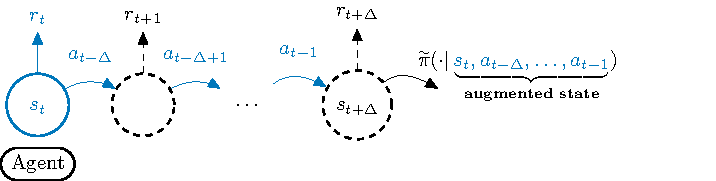
\includegraphics[bylabel=randomdelay]{img/thesis_plots.pdf}
    \caption{随机延迟示例：在时刻 $t$，延迟为 $n$；在时刻 $t+1$，延迟变为 $n'=n-1$。
    这意味着智能体观测到了 2 个新状态。
    步数之间的观测数量随机变量 $O$ 的概率定义为如\Cref{eq:observed} 所示概率的乘积。
    注意，索引 $t-n+1$ 的状态是否被观测到无关紧要，因为已观测到更近期的状态。}
    \label{fig:random_delay}
\end{figure}


该过程的奖励可定义如下，
\begin{align*}
    \augmentedexpectedrewardfunction(x,a) = \sum_{k=0}^{n}\probability(O=k)\sum_{i=0}^{k-1} \gamma^i\expectedvalue_{s_i\sim p^i(s_i\vert x,a)}[r(s_i,a_i)].
\end{align*}
该奖励基本上将新观测到的所有步数的奖励求和。
该定义假设，每当某个状态被观测到时，所有尚未观测到的中间状态将被同时观测到。

显然，涉及增广状态的过程定义了一个 \gls{mdp}，并证明了以下命题。

\begin{prop}
\label{pp:stoch_dmdp_is_mdp}
    具有独立同分布延迟 $(\delay_t)_{t\ge0}$（离散分布 $\zeta$，如上定义）的 \gls{dmdp} 可通过用最近的 $\delaymax$ 个动作和当前有效延迟增广状态来归结为 \gls{mdp}。
\end{prop}
该命题也在 \cite{bouteiller2020reinforcement} 中针对更一般的状态观测和动作执行延迟设定中被发现。
需要注意的是，包含动作执行延迟会带来一个问题：在给定时间步可能没有动作被执行，或者多个动作在同一时间步被执行。
在这些情况下，必须定义环境的行为。

现在考虑在此框架中应用 DIDA 学习的策略 $\delayedpolicy$，以研究当真实环境具有随机延迟但错误假设为常值延迟时的影响。
注意，DIDA 训练的常值 $\delay$-延迟 \gls{dmdp} 可视为上述过程的一个实例，其中 $\zeta$ 分布的全部权重放置在 $\delay$ 处。
在这种情况下，对于 $x = (s,a_1,\dots,a_\delaymax,n)$，认为 $\delayedpolicy(\cdot\vert x) = \delayedpolicy(\cdot\vert s,a_{\delaymax-\delay+1},\dots,a_\delaymax)$。
实际上，DIDA 将状态 $s$ 视为延迟了 $\delay$，并且对 $n$ 不可见。
将 DIDA 与如下定义的策略 $\widecheck{\pi}$ 进行比较：
\begin{align}
    \widecheck{\pi}(a\vert x) = \int_{\statespace} \augmentedbelief[n](s\vert x) \pi(a\vert s) \de s.\label{eq:belief_pol_stoch}
\end{align}
该策略的构造与 DIDA 相似，但适应 $n$ 的值。
下文中，记 $\widebar\delay$ 为随机延迟过程的平均延迟，定义如下：
\begin{align*}
    \widebar\delay = \expectedvalue[n] =  \sum_{k=0}^{\delaymax}k\prod_{i=0}^{k-1}\probability(\delay_i>i)\probability(\delay_k=k)
\end{align*}


\begin{thm}
\label{thm:stoch_mdp_dida_bound}
    考虑如上定义的具有随机延迟的 \gls{dmdp}，假设底层 \gls{mdp} 是 $L_T$-TLC 的。
    考虑由 DIDA 针对常值延迟学习的策略 $\delayedpolicy$（\Cref{eq:belief_pol}）和策略 $\widecheck\pi$（\Cref{eq:belief_pol_stoch}）。
    假设 $\delayedpolicy$ 的 Q 函数 $Q^\delayedpolicy$ 在第二个参数上是 $L_{\widetilde Q}$-LC 的\footnote{例如，当 $\gamma\max(L_P,1)\cdot(1+2L_\pi L_P)<1$ 时成立。该结果通过将 \cite[Theorem~1]{rachelson2010locality} 应用于常值延迟 \gls{mdp}（\Cref{pp:lip_dmdp}）和 DIDA 策略（\Cref{pp:lip_dida_pol}）的 Lipschitz 常数得到。}。
    则 $\delayedpolicy$ 和 $\widecheck\pi$ 之间的性能差异可界为：
    \begin{align*}
        \lvert V^{\widecheck{\pi}}(x)- V^{\delayedpolicy}(x)\rvert \le \frac{L_{\widetilde Q} L_\pi L_T }{1-\gamma}(\widebar\delay+\delay).
    \end{align*}
\end{thm}
\begin{proof}
    由\Cref{pp:stoch_dmdp_is_mdp}，随机延迟 \gls{dmdp} 是一个 \gls{mdp}。因此，可应用常规性能差异引理，对于 $x\in\widecheck{\augmentedstatespace}$\footnote{注意，本证明中，重载了原先定义于常值延迟 \gls{dmdp} 空间 $\augmentedstatespace$ 上的符号 $\delayeddiscountedstateoccupancydistribution[x][\delayedpolicy]$，改用空间 $\widecheck\augmentedstatespace$ 作为其定义域。}，
    \begin{align*}
        V^{\widecheck{\pi}}(x)- V^{\delayedpolicy}(x)
        = \frac{1}{1-\gamma} \expectedvalue_{x'\sim \delayeddiscountedstateoccupancydistribution[x][\widecheck\pi]} \left[\underbrace{V^{\delayedpolicy}(x) -  \expectedvalue_{a\sim \widecheck\pi(\cdot\vert x')}[Q^{\delayedpolicy}(x,a)]}_{A(x')}\right].
    \end{align*}
    如\Cref{th:perf_diff_bound} 中，可通过应用\Cref{pp:expected_q_bound} 推导以下界，其中记 $x'=(s',a_1',\dots,a_\delaymax',n')$，
    \begin{align}
        A(x')
        &\leq L_{\widetilde Q} \wassersteindistance(\widecheck\pi(\cdot\vert x')
        \Vert \delayedpolicy(\cdot\vert x'))
        \nonumber\\
        &= L_{\widetilde Q} \sup_{\left\Vert f\right\Vert_L\leq 1}\left\vert\int_{\actionspace} f(a)(\widecheck\pi(a\vert x')-\delayedpolicy(a\vert x') \de a\right\vert
        \nonumber\\
        &= L_{\widetilde Q} \sup_{\left\Vert f\right\Vert_L\leq 1}\left\vert\int_{\actionspace}\int_{\statespace} f(a)\pi(a\vert s)(\augmentedbelief[n'](s\vert x')-\augmentedbelief(s\vert x'))\de s  \de a\right\vert
        \nonumber\\
        &\leq L_{\widetilde Q} L_\pi \wassersteindistance(\augmentedbelief[n'](\cdot\vert x')
        \Vert \augmentedbelief(\cdot\vert x'))
        \nonumber\\
        &\leq L_{\widetilde Q} L_\pi L_T (n'+\delay),\label{eq:l_t_lip}
    \end{align}
    其中设定 $\augmentedbelief(s\vert x')=\augmentedbelief(s\vert s',a_1',\dots,a_\delaymax')$。这里使用了无延迟策略 $\pi$ 是 $L_{\pi}$-LC 的事实，\Cref{eq:l_t_lip} 通过复现\Cref{lem:bound_sigma_tlc} 的证明得到。
    因此，
    \begin{align*}
        V^{\widecheck{\pi}}(x)- V^{\delayedpolicy}(x)
        &\leq \frac{L_Q L_\pi L_T }{1-\gamma} \left(\delay +\expectedvalue_{x'\sim \delayeddiscountedstateoccupancydistribution[x][\widecheck\pi]}[n']\right)
        \\
        &= \frac{L_Q L_\pi L_T }{1-\gamma} \left(\delay +\widebar\delay\right),
    \end{align*}
    其中最后等式通过对增广状态中除 $n'$ 外的项积分得到。
\end{proof}

注意时间 Lipschitz 性质在证明中的重要性。
没有这一假设，$\wassersteindistance(\augmentedbelief[n'](\cdot\vert x')\Vert \augmentedbelief(\cdot\vert x'))$ 对 $x'$ 的依赖关系仍然存在，其在 $\delayeddiscountedstateoccupancydistribution[x][\widecheck\pi]$ 下的期望也不明确。
$n$ 与增广状态中其他元素之间确实存在非平凡依赖关系。
例如，当延迟较小时，$\statespace$ 中的某些状态可能被更频繁地访问。
另外注意，\Cref{th:perf_diff_bound} 中 $\statespace\subseteq\realnumbers^n$ 配备欧几里得范数的假设在此帮助不大，因为 $\wassersteindistance(\augmentedbelief[n'](\cdot\vert x')\Vert \augmentedbelief(\cdot\vert x'))$ 可能比较不同长度的轨迹（$n'\neq\delay$）。
DIDA 在该框架中对真实延迟不可见，构成了匿名延迟（anonymous delay）的情形（见\Cref{subsec:anonymous_delay_related}）。
据本文所知，这是 \gls{rl} 中匿名状态观测延迟的首个结果。

\section{实验评估}
\label{sec:exp_imitation}
本节提供实验以评估 DIDA 在广泛任务中的表现。
首先在\Cref{subsec:setting_exp_imitation} 中描述实验设置，然后在\Cref{subsec:results_imitation} 中展示并讨论结果。



\subsection{实验设置}
\label{subsec:setting_exp_imitation}

除 Trading 任务外，对所有任务运行 DIDA 和基线方法，取 10 个种子的结果进行平均。
Trading 任务的详细说明如下。

\subsubsection{任务}
\label{subsubsec:tasks_imitation}

\noindent\textbf{Pendulum。}\indent 与前一章相同，采用 Pendulum 环境，因其对延迟敏感。
考虑 $\{3, 5, 10, 15, 20\}$ 中的常值延迟。
对该任务，执行 500 个 epoch，每个 epoch 5,000 步，总计 250 万步。

\noindent\textbf{随机 Pendulum。}\indent 引入前一章定义的 Pendulum 随机版本，以评估 DIDA 在随机环境中的表现。
考虑常值延迟 5，执行 500 个 epoch，每个 epoch 5,000 步，总计 250 万步。

\noindent\textbf{非整数延迟 Pendulum。}\indent 为测试 DIDA 在非整数延迟上的表现，提出以下设置。
首先，学习一个持久度（persistence）为 2 的无延迟专家，其中持久度表示智能体在选择新动作之前重复执行同一动作的次数~\cite{metelli2020control}。
本质上，持久度为 2 时，智能体的控制频率减半。
DIDA 将在时间步集合 $(2t)_{t\in\naturalnumbers}$（与专家相同）中的状态下执行，而 DIDA 观测到的状态的时间步在 $(2t+1)_{t\in\naturalnumbers}$ 中。

\noindent\textbf{Mujoco。}\indent 类似地，引入四个 mujoco 环境：Walker2d、HalfCheetah、Reacher 和 Swimmer。
对这些任务，考虑常值延迟 5，执行 1,000 个 epoch，每个 epoch 5,000 步，总计 500 万步。

\noindent\textbf{Trading。}\indent 在该任务中，智能体以 10 分钟的控制频率交易 EUR-USD（\texteuro/\$）货币对，涵盖 2016-2019 年期间。
遵循 \cite{bisi2020foreign} 和 \cite{riva2021learning} 的框架，智能体相对于固定金额的 USD 可以选择买入（buy）、卖出（sell）或持平（flat）。
不考虑交易费用；但考虑买卖价差，其对奖励的影响在实践中等同于交易费用。
在该框架中，考虑 50 秒的常值动作执行延迟。
这导致非整数延迟。
在该任务中，使用 2016-2017 年数据训练不同方法，2018 年数据验证超参数，2019 年数据测试。
需要验证集是因为数据集由历史数据构成；
该任务是批量强化学习（batch \gls{rl}）或离线强化学习（offline \gls{rl}）任务，方法可能对训练集过拟合。

\noindent\textbf{同时学习多重延迟。}\indent 对于 Pendulum 和 mujoco 环境，同时评估 DIDA 在较大延迟上训练、在较小延迟上测试时的表现。
考虑在延迟 10 上训练 DIDA，然后在 $[\![1,9]\!]$ 的较小延迟上测试 Pendulum；类似地，在 mujoco 任务中，训练延迟为 5。


\subsubsection{基线方法}
考虑\Cref{subsubsec:baselines} 中使用的基线方法，采用相同超参数。
这些基线方法包括：无记忆 \gls{trpo}（M-TRPO）、增广状态 \gls{trpo}（A-TRPO）、增广状态 \gls{sac}（A-SAC）、无记忆 \gls{sac}（M-SAC）、SARSA 和 dSARSA（$\lambda=0.9$）。
同时包含之前的方法 L2-TRPO 和 D-TRPO。

同时考虑 M-DIDA（见\Cref{subsubsec:dida_no_undelayed_env}）作为基线，以评估是否需要访问无延迟环境。

对于 Trading 任务，用于训练 DIDA 的无延迟专家通过 2018 年的超参数验证选出。
也可以在延迟数据集上对 2018 年的超参数进行验证，以选择一个在延迟上泛化能力更强的专家（尽管是在无延迟数据上训练的）。
在实验中将此基线称为"延迟专家"（delayed expert）。

对于 Pendulum，还包含 BC-DIDA，对应于 DIDA 但使用行为克隆（behavioral cloning）~\cite{bain1995framework} 替代 \textsc{DAgger} 作为模仿算法。
该基线用于研究模仿算法选择的影响。


\subsubsection{DIDA 设置}
\label{subsubsection:our_approach_dida}
在所有实验中，为与其他基线进行公平的样本效率比较，将训练无延迟专家所需的步数纳入考虑，并相应平移 DIDA 的起始样本数。
在图中以垂直虚线表示。
关于无延迟专家本身，从前述理论可见，更平滑的专家对模仿延迟策略的性能界有利（\Cref{th:perf_diff_bound}）。
因此，除 Trading 任务外，所有实验均采用 \gls{sac} 作为专家。
关于平滑策略的研究~\cite{mysore2021regularizing} 表明，\gls{sac} 的熵正则化框架在实践中具有学习更平滑策略的效果，而无需显式优化策略的平滑性。
对于 DIDA 自身的策略，使用简单的前馈神经网络。

对于 Trading 环境，利用通过 Fitted Q-Iteration（FQI）~\cite{ernst2005tree} 在 2016-2017 年数据上训练的专家知识，使用 XGBoost~\cite{chen2016xgboost} 作为 $Q$ 函数的回归器，与 \cite{riva2022addressing} 中的方法相同。
在该任务中，为更好地匹配专家的基于树的方法，使用 Extra Trees~\cite{geurts2006extremely} 作为 DIDA 的策略。
该环境高度随机，使用不同种子训练的专家可能具有非常不同的性能。
因此，考虑 4 个使用不同种子但相同配置训练的专家。
对每个专家，使用 5 个种子重复 DIDA 的训练。
总计 20 次 DIDA 试验，对其结果计算均值和标准差。

对于 $\beta$-routine，如 \cite{ross2011reduction} 建议，设置 $\beta_1=1, \beta_{i\ge 2}=0$。
这意味着无延迟专家仅在 DIDA 的第一次迭代中用于从环境采样。

如\Cref{algo:dida} 所示，每次迭代中，DIDA 训练的示例缓冲区会加入最新样本。为防止无限增长，使用最大缓冲区大小为 10 次迭代。
这意味着当缓冲区满时，较新的样本会以先进先出的方式覆盖最旧的样本。



\subsection{实验结果}
\label{subsec:results_imitation}

\noindent\textbf{Pendulum。}\indent 不同延迟值下各方法的回报如\Cref{fig:pendulum_varying_delay_imitation} 所示。
对于小延迟，DIDA、BC-DIDA 和 M-DIDA 取得的回报与 A-SAC 相当，略优于 D-TRPO 和 L2-TRPO。
当延迟增加时观察到有趣的现象。
显然，DIDA 和 M-DIDA 对所有其他基线以及 BC-DIDA 对延迟增加更为鲁棒，BC-DIDA 的性能急剧下降。
值得注意的是 DIDA 和 M-DIDA 性能相似，这表明从无延迟环境采样并非算法的关键要素。
\Cref{fig:pendulum_imitation} 中聚焦延迟 5 的结果证实了这一点，该图展示了性能随样本数的变化。
DIDA 和 M-DIDA 在所需样本数方面具有非常相似的学习速度，而 BC-DIDA 稍慢，A-SAC 也稍慢。
专家策略与 DIDA 之间的性能差异源于\Cref{subsec:delay_init} 中提及的延迟初始化偏移问题。
在初始步骤中，为在实践中初始化延迟环境，动作从环境中均匀随机采样，这可能迫使智能体在与真实初始状态相比不利的状态下开始动作。

\begin{figure}[t]
    \centering
    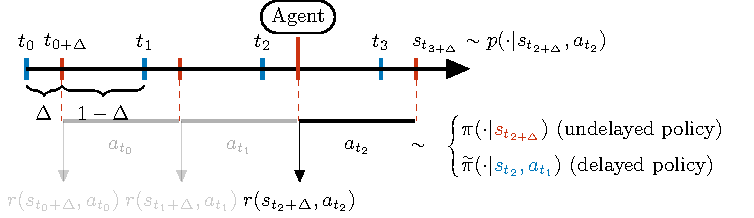
\includegraphics[labelimitation=pendulumvaryingdelay]{img/thesis_plots_imitation.pdf}
    \caption{DIDA 和基线方法在 Pendulum 环境中不同延迟值下的平均回报。
    水平虚线对应无延迟专家（\gls{sac}）的性能。
    阴影区域表示一个标准差，结果基于 10 个种子获得。}
    \label{fig:pendulum_varying_delay_imitation}
\end{figure}

\begin{figure}[t]
    \centering
    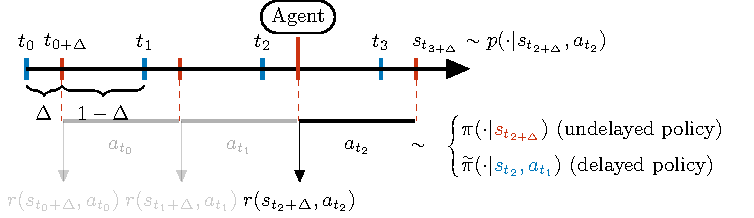
\includegraphics[labelimitation=delay5pendulumimitation]{img/thesis_plots_imitation.pdf}
    \caption{DIDA 和基准方法在 Pendulum 环境中延迟为 5 时获得的回报。
    水平虚线对应专家的回报，垂直虚线表示训练专家所用的步数。
    阴影区域表示一个标准差，结果基于 10 个种子获得。}
    \label{fig:pendulum_imitation}
\end{figure}

\noindent\textbf{随机 Pendulum。}\indent 这些任务的结果如\Cref{fig:noise_pendulum_imitation} 所示。
与前一章相同，噪声按照\Cref{tab:noises} 分为几组。
在左上图中，所有噪声均基于 beta 分布。
在该任务中，DIDA 不仅取得了远优于基线的最终性能，而且收敛到这些性能的速度也远快于基线。
在右上图的第二组中，基线性能接近 DIDA，但 DIDA 仍然显著领先。
最后，在左下图的第三组中，DIDA 再次取得最佳性能。
对于 LogNormal(1.0) 噪声，即使 DIDA 的性能也显著下降，这在意料之中，因为该噪声高度不对称，使信念分布对算法更具挑战性。

\begin{figure}[t]
    \centering
    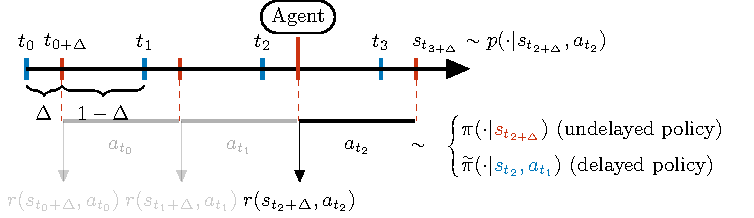
\includegraphics[labelimitation=pendulumnoiseimitation]{img/thesis_plots_imitation.pdf}
    \caption{添加不同噪声（如\Cref{tab:noises} 所述）的 Pendulum 环境中 DIDA 和基线方法获得的回报。
    颜色表示噪声类型，标记表示算法。
    水平虚线表示每种噪声下专家的回报，垂直虚线表示训练专家所用的步数。
    在右上图中，专家性能汇聚在一起。
    阴影区域表示一个标准差，结果基于 10 个种子获得。}
    \label{fig:noise_pendulum_imitation}
\end{figure}

\noindent\textbf{非整数延迟 Pendulum。}\indent 结果如\Cref{fig:pendulum_non_int_imitation} 所示。
在该任务中，DIDA 的性能略低于其在整数延迟上的性能（报告于\Cref{fig:pendulum_varying_delay_imitation}）。
有两个原因。
首先，专家以持久度 2 训练，回报略低。
其次，此处 DIDA 将其动作持续执行 2 步，因此延迟值也翻倍。
\Cref{fig:pendulum_non_int_imitation} 中的延迟 1 对应于\Cref{fig:pendulum_varying_delay_imitation} 中的延迟 2。
无论如何，DIDA 的性能仍然令人满意，表明其能够有效适应非整数延迟。

\begin{figure}[t]
    \centering
    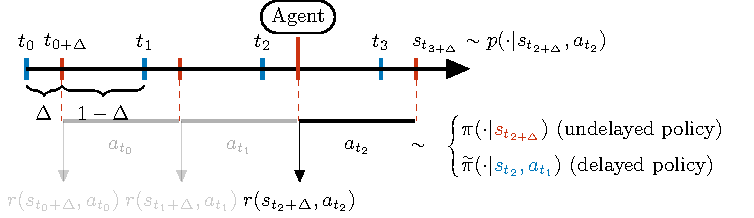
\includegraphics[labelimitation=pendulumnonint]{img/thesis_plots_imitation.pdf}
    \caption{DIDA 在 Pendulum 环境中不同非整数延迟值下的平均回报。
    水平虚线表示无延迟专家（\gls{sac}）的性能。
    阴影区域表示一个标准差，结果基于 10 个种子获得。}
    \label{fig:pendulum_non_int_imitation}
\end{figure}

\noindent\textbf{Mujoco。}\indent 结果如\Cref{fig:mujoco_imitation} 所示。
此处再次，DIDA 和 M-DIDA 取得了相似性能，同时优于所有基线。
部分由于延迟的初始化偏移，在 HalfCheetah 和 Reacher 中，DIDA 的表现远差于无延迟专家。
更令人惊讶的是，在 Swimmer 中，DIDA 的表现略好于专家。
这是延迟初始化偏移的一个意外后果。
事实上，在某些环境中，初始随机动作序列可能将智能体置于有利状态。
在 HalfCheetah 中，随机动作有时使智能体头朝下，因此必须先站起来才能移动。而在 Swimmer 中，随机动作为智能体提供了初始速度。

\begin{figure}[t]
    \centering
    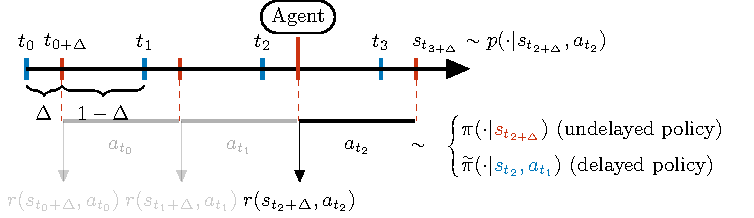
\includegraphics[labelimitation=delay5mujocoimitation]{img/thesis_plots_imitation.pdf}
    \caption{DIDA 和基准方法在各种 Mujoco 环境中获得的回报。
    水平虚线对应专家的回报，垂直虚线表示训练专家所用的步数。
    阴影区域表示一个标准差，结果基于 10 个种子获得。}
    \label{fig:mujoco_imitation}
\end{figure}

\noindent\textbf{Trading。}\indent 对于该任务，报告训练集（2019）上获得的结果，如\Cref{fig:trading_dida} 所示。
鉴于买卖价差的存在对回报具有决定性影响，仅获得正回报便已是不小的成就。
DIDA 不仅取得了正回报，而且明显优于延迟专家。
令人惊讶的一点是，DIDA 初始时获得了比专家本身更好的回报。
策略实际上略有不同。
在\Cref{fig:allocation} 中，通过表示 DIDA 学习到的策略与专家策略的动作模式对比，分析 DIDA 学习到的策略。
具体来说，该图说明了批量 RL 设定的困难。
DIDA 在第 10 次迭代学习到的策略与训练集上的专家非常相似，但开始偏离测试集上的专家。

\begin{figure}[t]
    \centering
    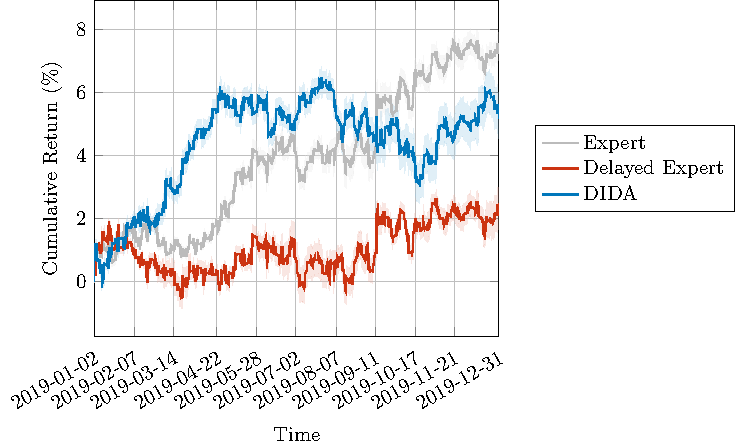
\includegraphics[labelimitationtrading=didatradingeurusd]{img/thesis_plots_chapter_imitation_trading.pdf}
    \caption{2019 年 EUR-USD 货币对交易的累计回报（占投资金额的百分比）。
    DIDA 与其训练的专家以及一个超参数在延迟数据集上选择的无延迟专家（称为"延迟专家"）进行比较。}
    \label{fig:trading_dida}
\end{figure}


\begin{figure*}[t]
\centering
    \begin{subfigure}{0.33\textwidth}
        \centering
        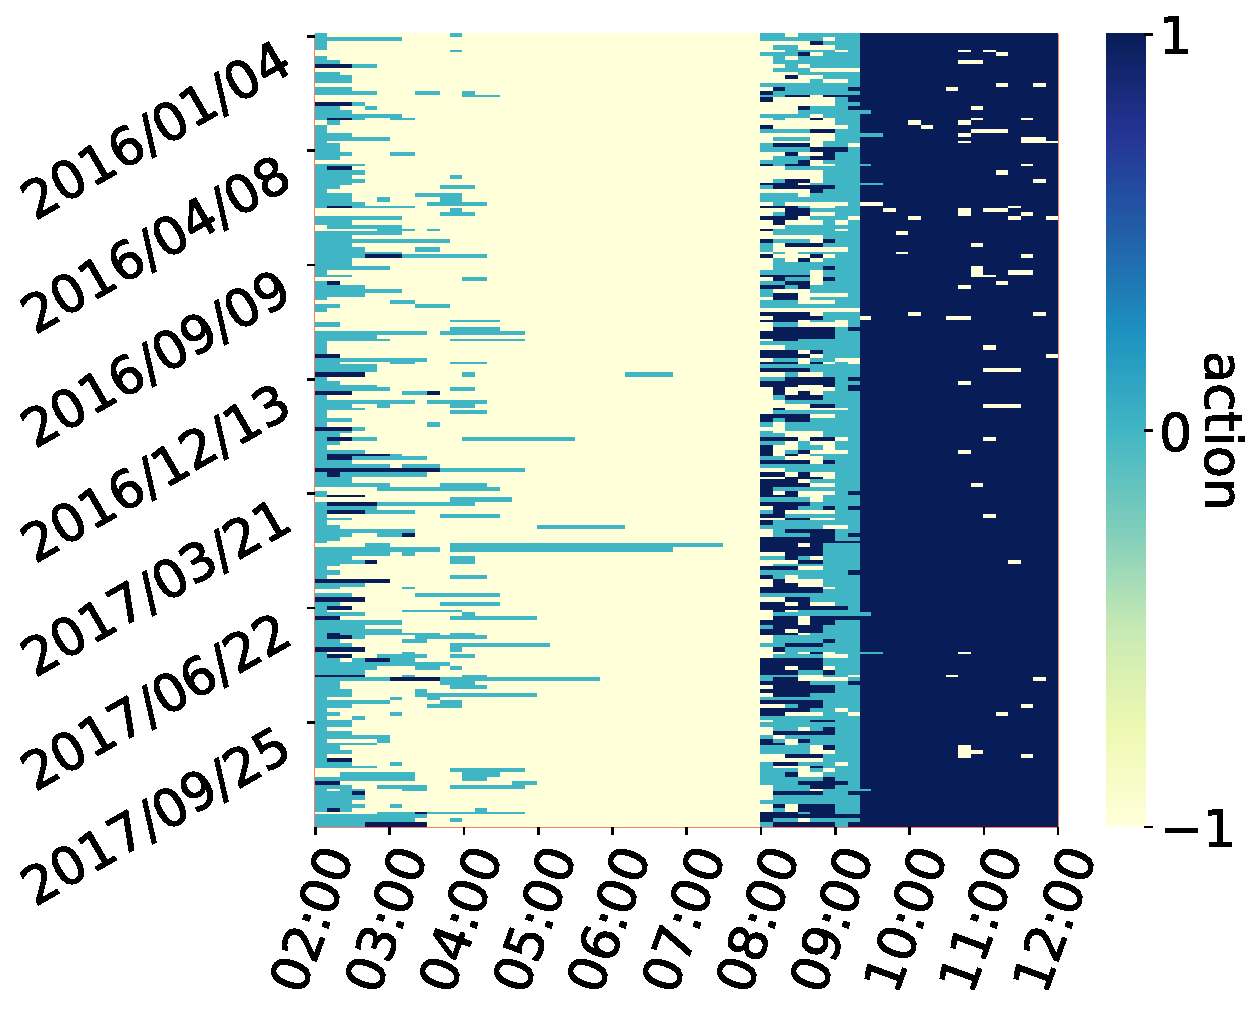
\includegraphics[width=\linewidth]{img/imitation/expert_2016_2017_regular_shift50_expite_10_expseed_0_allocations.pdf}
        \caption{专家，2016-2017。}
        \label{fig:test_expert_fx_allocation}
    \end{subfigure}%
\hfill
    \begin{subfigure}{0.33\textwidth}
        \centering
        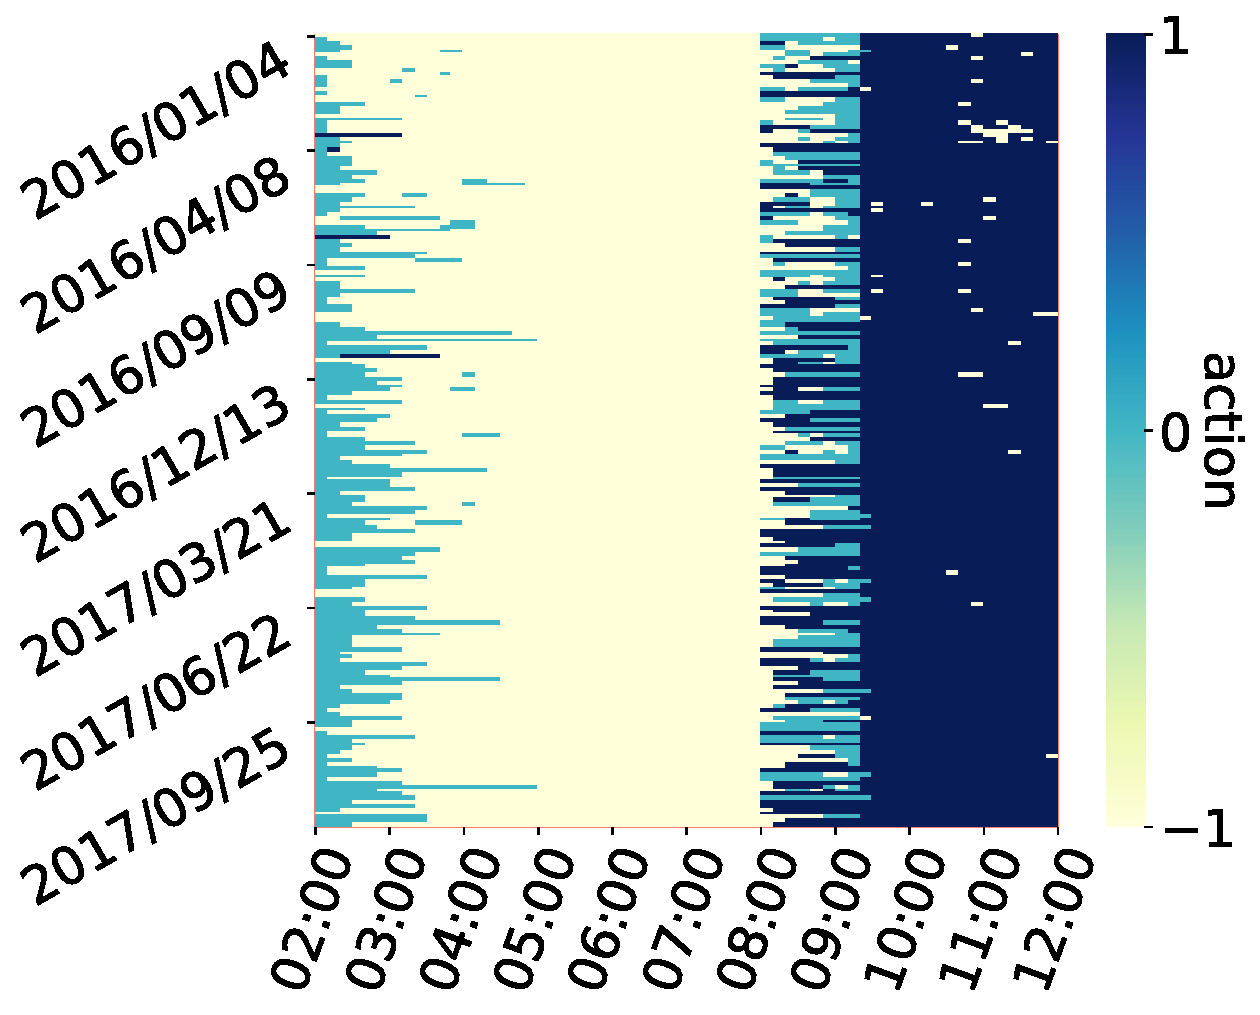
\includegraphics[width=\linewidth]{img/imitation/dida_ms100_est100_shift50_2016_2017_expite_10_expseed_0_dagite_10_dagseed1_allocations.pdf}
        \caption{DIDA，2016-2017。}
        \label{fig:train_dida_fx_allocation}
    \end{subfigure}%
    \begin{subfigure}{0.33\textwidth}
        \centering
        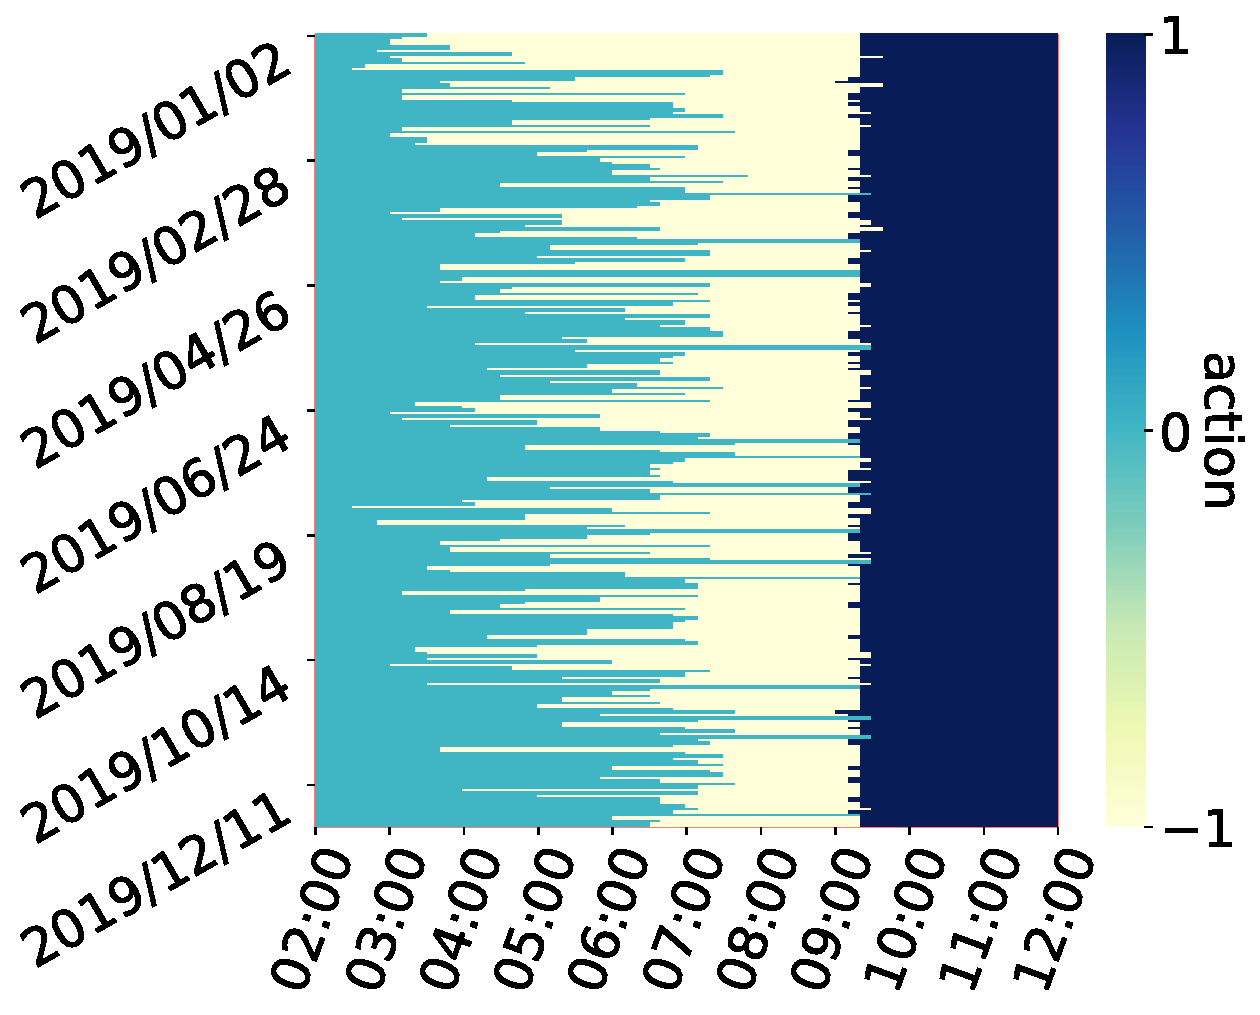
\includegraphics[width=\linewidth]{img/imitation/dida_ms100_est100_shift50_2019_expite_10_expseed_0_dagite_10_dagseed1_allocations.pdf}
        \caption{DIDA，2019。}
        \label{fig:test_dida_fx_allocation}
    \end{subfigure}%
\caption{表示 Trading 任务中专家的动作模式和 DIDA 的动作模式的热力图。
将专家的动作模式（左）与 DIDA 在第 10 次迭代的动作模式进行比较，分别在训练集（2016-2017，中）和测试集（2019，右）上。
热力图显示给定天（行）的给定分钟（列）所选的动作（颜色）。}
\label{fig:allocation}
\end{figure*}

\noindent\textbf{同时学习多重延迟。}\indent 此处探索\Cref{subsubsec:multi_delay_once_imitation} 中提出的思路，即将 DIDA 针对某个延迟 $\delay>0$ 学习的策略应用于更小的延迟 $0<\delay'<\delay$。
在\Cref{fig:pendulum_multi_delay_imitation} 中，给出 Pendulum 任务的结果，其中 DIDA 策略在延迟 $\delay=10$ 上训练。
在\Cref{fig:mujoco_multi_delay_imitation} 中，给出 mujoco 任务的结果，其中 DIDA 策略在延迟 $\delay=5$ 上训练。
显然且符合预期，在较小延迟上获得的性能与 DIDA 在训练所用延迟上达到的性能相似。



\begin{figure}[t]
    \centering
    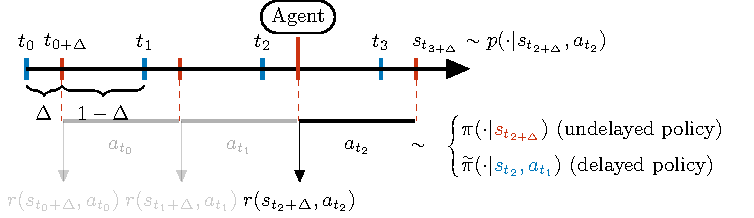
\includegraphics[labelimitation=multipledelayspendulumimitation]{img/thesis_plots_imitation.pdf}
    \caption{在 Pendulum 上，以延迟 10 训练的 DIDA 在较小延迟上测试获得的回报。}
    \label{fig:pendulum_multi_delay_imitation}
\end{figure}

\begin{figure}[t]
    \centering
    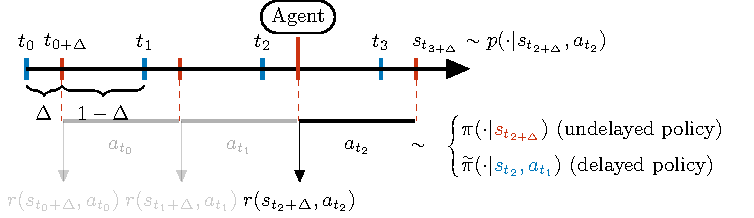
\includegraphics[labelimitation=multipledelaysmujocoimitation]{img/thesis_plots_imitation.pdf}
    \caption{在多种 Mujoco 环境中，以延迟 5 训练的 DIDA 在较小延迟上测试获得的回报。}
    \label{fig:mujoco_multi_delay_imitation}
\end{figure}

\section{结论}
本章针对状态观测或动作执行中的常值延迟问题，设计了一种简单而高效的解决方案。
该方案首先在无延迟环境中学习一个策略，然后在延迟环境中模仿该策略。
本文证明了在环境具有平滑性时，此类模仿策略相对于无延迟专家的性能界。
利用这些理论洞见，设计了 DIDA 算法，该算法遵循上述原则，采用 \textsc{DAgger} 作为模仿算法。
实验结果展示了 DIDA 相对于众多基线方法的有效性。
DIDA 几乎总能取得更优的回报，同时需要更少的样本。
有趣的是，本文展示了该算法如何经过修改适用于另外三种场景。
首先，当延迟为常值但非整数时，对 DIDA 进行简单调整即表现出良好的实验结果。
其次，虽然 DIDA 是在常值延迟上训练的，但本文为其在随机延迟上测试时提供了理论保证。
第三，将\Cref{chap:belief_based} 中的简单"技巧"应用于 DIDA，可利用针对某一延迟学习的策略高效地应用于更小延迟。
作为未来研究方向，可修改当前算法使其在随机延迟上训练，并学习\Cref{eq:belief_pol_stoch} 中的策略。
这样将获得比\Cref{thm:stoch_mdp_dida_bound} 提供更好的理论保证。
另一个方向是解决 DIDA 的主要缺点——对无延迟专家的依赖。
一种可能的思路是从延迟策略收集的数据集中离线学习一个无延迟专家。
这意味着不再需要从无延迟环境中采样任何样本。

